
\chapter{Projeto da Interação Humano-Computador}
\label{sec-ihc}
\vspace{-1cm}

% Permite quebrar melhor os parágrafos com identificadores longos em fonte monoespaçada.
\emergencystretch=3em

% Inclui a figura se o arquivo existir; senão, mostra uma caixa de aviso.
\providecommand{\figciu}[2]{%
	\IfFileExists{#1}{%
		\includegraphics[width=1\textwidth,height=#2\textheight,keepaspectratio]{#1}%
	}{%
		\fbox{\parbox{0.9\textwidth}{\centering\vspace{3cm}\textbf{[Diagrama pendente]}\\[2pt]\texttt{#1}\vspace{3cm}}}%
	}%
}

Este capítulo apresenta o projeto da Camada de Apresentação dos três subsistemas do Happy Paws: Gestão de Perfis, Serviços e Suporte (Figura~\ref{figura-arquitetura}). Na Camada de Apresentação é feita a comunicação entre as pessoas e o sistema: ela define como o usuário comanda o sistema e como o sistema mostra as informações a ele~\cite{falbo:notas18}.


%=======================================================================================================
\section{Organização da Camada de Apresentação}
\label{sec-ihc-organizacao}

Na Camada de Apresentação foi aplicado o padrão Modelo-Visão-Controlador (\textit{Model-View-Controller}, MVC), em que a lógica de negócio (Capítulo~\ref{sec-logica-negocio}) faz o papel do Modelo. Seguindo Falbo~\cite{falbo:notas18}, a Camada de Interface com o Usuário (CIU) de cada subsistema é dividida em dois pacotes, que correspondem às componentes da Tabela~\ref{tabela-pacotes-ciu}: o pacote \texttt{cih}, com a Componente de Interação Humana (CIH), que contém as páginas e os elementos visuais; e o pacote \texttt{cci}, com a Componente de Controle de Interação (CCI), que contém as classes que recebem as requisições das páginas, chamam as classes de aplicação do \texttt{cgt} e decidem qual página mostrar em seguida.

\begin{footnotesize}
\setlength{\tabcolsep}{4pt}
\begin{longtable}{|c|p{4.8cm}|p{6.2cm}|}
	\caption{Pacotes da Camada de Apresentação e as componentes equivalentes em~\cite{falbo:notas18}.}
	\label{tabela-pacotes-ciu}\\\hline
	\rowcolor{lightgray}
	\textbf{Pacote} & \textbf{Componente} & \textbf{Implementação no Happy Paws} \\\hline
	\endfirsthead
	\hline
	\rowcolor{lightgray}
	\textbf{Pacote} & \textbf{Componente} & \textbf{Implementação no Happy Paws} \\\hline
	\endhead
	\texttt{cih} & Componente de Interação Humana (CIH) & Páginas do Next.js e componentes React (shadcn/ui e Tailwind CSS), incluindo os componentes executados no navegador, como o mapa e a captura de GPS \\\hline
	\texttt{cci} & Componente de Controle de Interação (CCI) & Módulos de \textit{Server Actions} (comandos) e funções de consulta chamadas pelas páginas, e \textit{Route Handlers} para o envio de eventos em tempo real \\\hline
\end{longtable}
\end{footnotesize}

O pacote \texttt{cih} e o pacote \texttt{cci} são interdependentes, pois uma página envia dados e comandos ao controlador e recebe dele os dados a mostrar. Já o pacote \texttt{cci} depende, de um lado só, do pacote \texttt{cgt}: as classes de aplicação (\texttt{Apl*}) não conhecem a Camada de Apresentação, o que mantém a lógica de negócio independente da interface (Capítulo~\ref{sec-logica-negocio}). Toda chamada da interface à lógica de negócio passa por um controlador; nenhuma página chama diretamente uma classe \texttt{Apl*} ou um repositório.

Os diagramas das próximas seções seguem esta notação:

\begin{itemize}
	\item Elementos com o ícone de objeto de interface (estereótipo \texttt{<<boundary>>}) representam as páginas (rotas) do sistema e, quando for importante para o projeto, componentes de página executados no navegador, como o mapa do passeio;
	\item Elementos com o ícone de controlador de interação (estereótipo \texttt{<<control>>}) representam os controladores do pacote \texttt{cci}. Os nomes terminam com \texttt{Controller}. Cada controlador é implementado como um módulo de \textit{Server Actions} do Next.js (as operações que alteram dados) junto com as funções de consulta usadas pelas páginas. A exceção são os controladores terminados em \texttt{Handler}, que são \textit{Route Handlers} do Next.js e servem eventos em tempo real por \textit{Server-Sent Events} (SSE);
	\item Classes com o estereótipo \texttt{<<interface>>} representam, com suas operações, as classes de aplicação do pacote \texttt{cgt}, que são a porta de entrada da Camada de Negócio, e a interface \texttt{NotificadorTempoReal};
	\item Uma associação bidirecional entre página e controlador indica a ligação entre os campos e botões da página e as operações do controlador: os dados vão e voltam (formulários enviados a \textit{Server Actions} e dados de consulta mostrados na página);
	\item Uma associação unidirecional do controlador para a página indica um redirecionamento: como resultado de uma operação, o controlador manda o usuário para outra página, sem trocar dados com ela;
	\item Uma associação unidirecional entre páginas indica um \textit{link} (navegação) para a página de destino;
	\item As cardinalidades aparecem apenas nas associações entre controladores e classes de aplicação, no lado navegável (da classe de aplicação). As demais associações envolvem páginas e não têm cardinalidade;
	\item Setas tracejadas entre classes do \texttt{cgt} indicam dependência (por exemplo, de uma classe de aplicação para \texttt{NotificadorTempoReal}), como nos diagramas do Capítulo~\ref{sec-logica-negocio};
	\item O losango cheio indica composição: um componente executado no navegador que faz parte de uma página (\texttt{RastreadorGps} em \texttt{ExecucaoPasseioPage});
	\item \textit{Links} presentes em todas as páginas de uma área, como os do menu do \textit{layout}, não são desenhados, para não poluir os diagramas;
	\item Cada diagrama mostra um único subsistema, por isso os \textit{links} para páginas de outro subsistema também não são desenhados e são descritos no texto (por exemplo, de \texttt{AcompanhamentoPasseioPage}, de Serviços, para \texttt{AbrirChamadoPage}, de Suporte).
\end{itemize}

Quanto aos nomes, as classes de aplicação mantêm o prefixo \texttt{Apl} do padrão do prof. Falbo~\cite{falbo:notas18}. Na Camada de Apresentação foi usado o padrão comum em aplicações React e Next.js, em que o sufixo indica o tipo de artefato da plataforma: as páginas terminam em \texttt{Page}, os controladores (\textit{Server Actions}) em \texttt{Controller} e os \textit{Route Handlers} em \texttt{Handler}, no lugar dos prefixos \texttt{Jan}/\texttt{Painel} e \texttt{Ctrl} sugeridos por Falbo.


%=======================================================================================================
\section{Perfis de Usuário e Táticas de Usabilidade}
\label{sec-ihc-usabilidade}

O Happy Paws tem três perfis de usuário (Tutor, Passeador e Atendente) e um visitante ainda não cadastrado, e cada um usa o sistema em uma situação diferente, o que influencia o projeto das páginas:

\begin{itemize}
	\item \textbf{Tutor:} usa o sistema de forma ocasional, na maioria das vezes pelo celular, e não domina a tecnologia. As páginas precisam ser simples, com poucos campos e sem termos técnicos;
	\item \textbf{Passeador:} usa o sistema em movimento e ao ar livre, muitas vezes com uma mão só e sob luz do sol. As páginas de execução do passeio têm poucos comandos, botões grandes, bom contraste e não exigem digitação longa;
	\item \textbf{Atendente:} usa o sistema todos os dias, em um computador, e trata muitos chamados e validações. As páginas mostram listas ordenadas e com o estado de cada item à vista, para reduzir o número de ações.
\end{itemize}

A Tabela~\ref{tabela-matriz-us-perfil} mostra quais perfis têm acesso a cada \textit{user story}, em uma matriz \textit{user story} $\times$ perfil~\cite{falbo:notas18}. As Server Actions e o layout de cada área verificam a sessão (Better Auth) e o perfil do usuário antes de executar a operação e de mostrar a página, conforme o RNF-2.

\begin{footnotesize}
\setlength{\tabcolsep}{4pt}
\begin{longtable}{|p{1cm}|p{5cm}|c|c|c|c|}
	\caption{Matriz \textit{user story} $\times$ perfil de usuário.}
	\label{tabela-matriz-us-perfil}\\\hline
	\rowcolor{lightgray}
	\textbf{US} & \textbf{Funcionalidade} & \textbf{Visitante} & \textbf{Tutor} & \textbf{Passeador} & \textbf{Atendente} \\\hline
	\endfirsthead
	\hline
	\rowcolor{lightgray}
	\textbf{US} & \textbf{Funcionalidade} & \textbf{Visitante} & \textbf{Tutor} & \textbf{Passeador} & \textbf{Atendente} \\\hline
	\endhead
	% Títulos conferidos com as user stories do Documento de Especificação de Requisitos (seção 4.1).
	US01 & Cadastrar dados pessoais e perfil do Tutor & X & X & & \\\hline
	US02 & Cadastrar o perfil do cão & & X & & \\\hline
	US03 & Cadastrar dados profissionais do Passeador & X & & X & \\\hline
	US04 & Obter o status de perfil validado & & & X & X \\\hline
	US05 & Compartilhar o perfil do cão para gestão conjunta & & X & & \\\hline
	US06 & Definir o modo de trabalho & & & X & \\\hline
	US07 & Pesquisar passeadores & & X & & \\\hline
	US08 & Agendar um passeio único & & X & X & \\\hline
	US09 & Agendar passeios em dias fixos & & X & X & \\\hline
	US10 & Visualizar o trajeto do passeio via GPS & & X & & \\\hline
	US11 & Iniciar e finalizar o passeio & & & X & \\\hline
	US12 & Postar fotos do cão no mural & & & X & \\\hline
	US13 & Visualizar as fotos e conquistas do cão & & X & & \\\hline
	US14 & Realizar o pagamento do passeio & & X & & \\\hline
	US15 & Avaliar o serviço do passeador & & X & & \\\hline
	US16 & Registrar um chamado de suporte & & X & X & \\\hline
	US17 & Responder aos chamados de suporte & & & & X \\\hline
\end{longtable}
\end{footnotesize}

A Tabela~\ref{tabela-taticas-usabilidade} mostra as táticas de usabilidade~\cite{falbo:notas18} aplicadas às páginas, relacionadas aos requisitos não funcionais do Capítulo~\ref{sec-rnfs}.

\begin{footnotesize}
\setlength{\tabcolsep}{4pt}
\begin{longtable}{|p{4.2cm}|p{10.2cm}|}
	\caption{Táticas de usabilidade aplicadas à Camada de Apresentação.}
	\label{tabela-taticas-usabilidade}\\\hline
	\rowcolor{lightgray}
	\textbf{Tática} & \textbf{Aplicação no Happy Paws} \\\hline
	\endfirsthead
	\hline
	\rowcolor{lightgray}
	\textbf{Tática} & \textbf{Aplicação no Happy Paws} \\\hline
	\endhead
	Separar a interface do restante da aplicação & Padrão MVC com os pacotes \texttt{cih} e \texttt{cci}, independentes do pacote \texttt{cgt} (Seção~\ref{sec-ihc-organizacao}). \\\hline
	Adotar padrões de interface conhecidos & Componentes shadcn/ui (formulários, listas, diálogos, abas, \textit{toasts}) e Tailwind CSS com abordagem \textit{mobile-first}, para a interface funcionar nos navegadores e telas alvo do RNF-1. \\\hline
	Entrada por seleção em vez de digitação & Os tipos enumerados da Camada de Negócio viram listas de seleção, botões de opção ou \textit{checkboxes}: porte, especialidade, tipo de documento, tipo de agendamento, dias da semana, método de pagamento e tipo de chamado. \\\hline
	Não exigir dados que o sistema obtém sozinho & A posição do Passeador é capturada pela \textit{Geolocation API}, sem digitação (RNF-5); o protocolo do chamado, o valor do agendamento e as datas de cadastro são gerados pelo sistema. \\\hline
	Feedback sobre o estado do sistema & Indicador de carregamento e botão desabilitado enquanto uma \textit{Server Action} está em andamento, mensagem de sucesso após cada operação e indicação de conexão em tempo real nas páginas de acompanhamento e de execução do passeio. \\\hline
	Mensagens de erro e aviso significativas & Os erros de regra de negócio (por exemplo, CPF já cadastrado, horário em conflito, limite de cães do Passeador) voltam do controlador para a página e são mostrados junto ao campo ou ao comando que os causou, em linguagem do usuário. \\\hline
	Confirmação para ações destrutivas & Diálogo de confirmação antes de cancelar um agendamento (que estorna o pagamento), remover um cão ou desvincular um Tutor, recusar uma validação e encerrar um chamado. \\\hline
	Desativar comandos inapropriados & O botão ``Iniciar passeio'' fica desativado enquanto o pagamento não estiver confirmado ou o horário previsto não tiver chegado; o botão ``Concluir'' só aparece com o passeio iniciado; a avaliação só é oferecida para passeios concluídos. \\\hline
	Priorização pelo sistema (iniciativa do sistema) & A fila de atendimento mostra os chamados de ``Emergência'' em destaque e no topo, com o tempo de espera de cada chamado (RNF-4). \\\hline
	Comandos para diferentes perfis & Cada perfil tem sua própria área e seu próprio menu, com só as funcionalidades da Tabela~\ref{tabela-matriz-us-perfil}. \\\hline
	Eficiência no uso de recursos do aparelho & A captura de GPS só funciona com o passeio iniciado e envia posições em intervalo mínimo, para economizar bateria (RNF-5). \\\hline
\end{longtable}
\end{footnotesize}


%=======================================================================================================
% ==============================================================================
% Projeto de Sistema - Happy Paws
% Capítulo 7, seção do protótipo de alta fidelidade (T3).
% Incluída por ch7-human-computer-interaction.tex, logo após a seção de perfis de
% usuário e táticas de usabilidade.
% ==============================================================================

\section{Protótipo de Alta Fidelidade}
\label{sec-ihc-prototipo}

Na disciplina de Engenharia de Software I foi construído um protótipo navegável do sistema, cujas telas aparecem nas Figuras 1 a 30 do Documento de Especificação de Requisitos. Como parte do projeto da interação humano-computador, esse protótipo foi revisto e redesenhado em alta fidelidade de acordo com as decisões deste capítulo: cada tela do protótipo corresponde agora a uma página do pacote \texttt{cih} (Tabelas~\ref{tabela-ciu-perfis}, \ref{tabela-ciu-servicos} e~\ref{tabela-ciu-suporte}) e aplica as táticas de usabilidade da Tabela~\ref{tabela-taticas-usabilidade}, detalhando as telas apresentadas no Documento de Especificação de Requisitos. A versão de Engenharia de Software I, com o visual anterior a esta revisão, continua em \url{https://happypawss.lovable.app}, mas as telas que valem para este projeto são as desta seção, publicadas no endereço indicado ao final dela.

As telas dos perfis Tutor e Passeador foram projetadas na largura de referência de 375~px (celular) e as do perfil Atendente na largura de 1180~px (navegador em um computador), de acordo com os perfis de usuário da Seção~\ref{sec-ihc-usabilidade} e com o RNF-1. Cada tela é identificada pelo nome da página do pacote \texttt{cih} e pela sua rota, o que mantém a rastreabilidade entre o protótipo, os diagramas da Camada de Interface com o Usuário e as tabelas de páginas. Os valores exibidos nas telas são os dos tipos enumerados da Camada de Negócio (Tabela~\ref{tabela-enumerados}) e os das mensagens definidas nos critérios de aceitação do Documento de Especificação de Requisitos.

As Figuras~\ref{figura-proto-perfis-1} a~\ref{figura-proto-validacao} apresentam o protótipo, organizado por subsistema.

% ------------------------------------------------------ Gestão de Perfis
\begin{figure}[htbp]
	\centering
	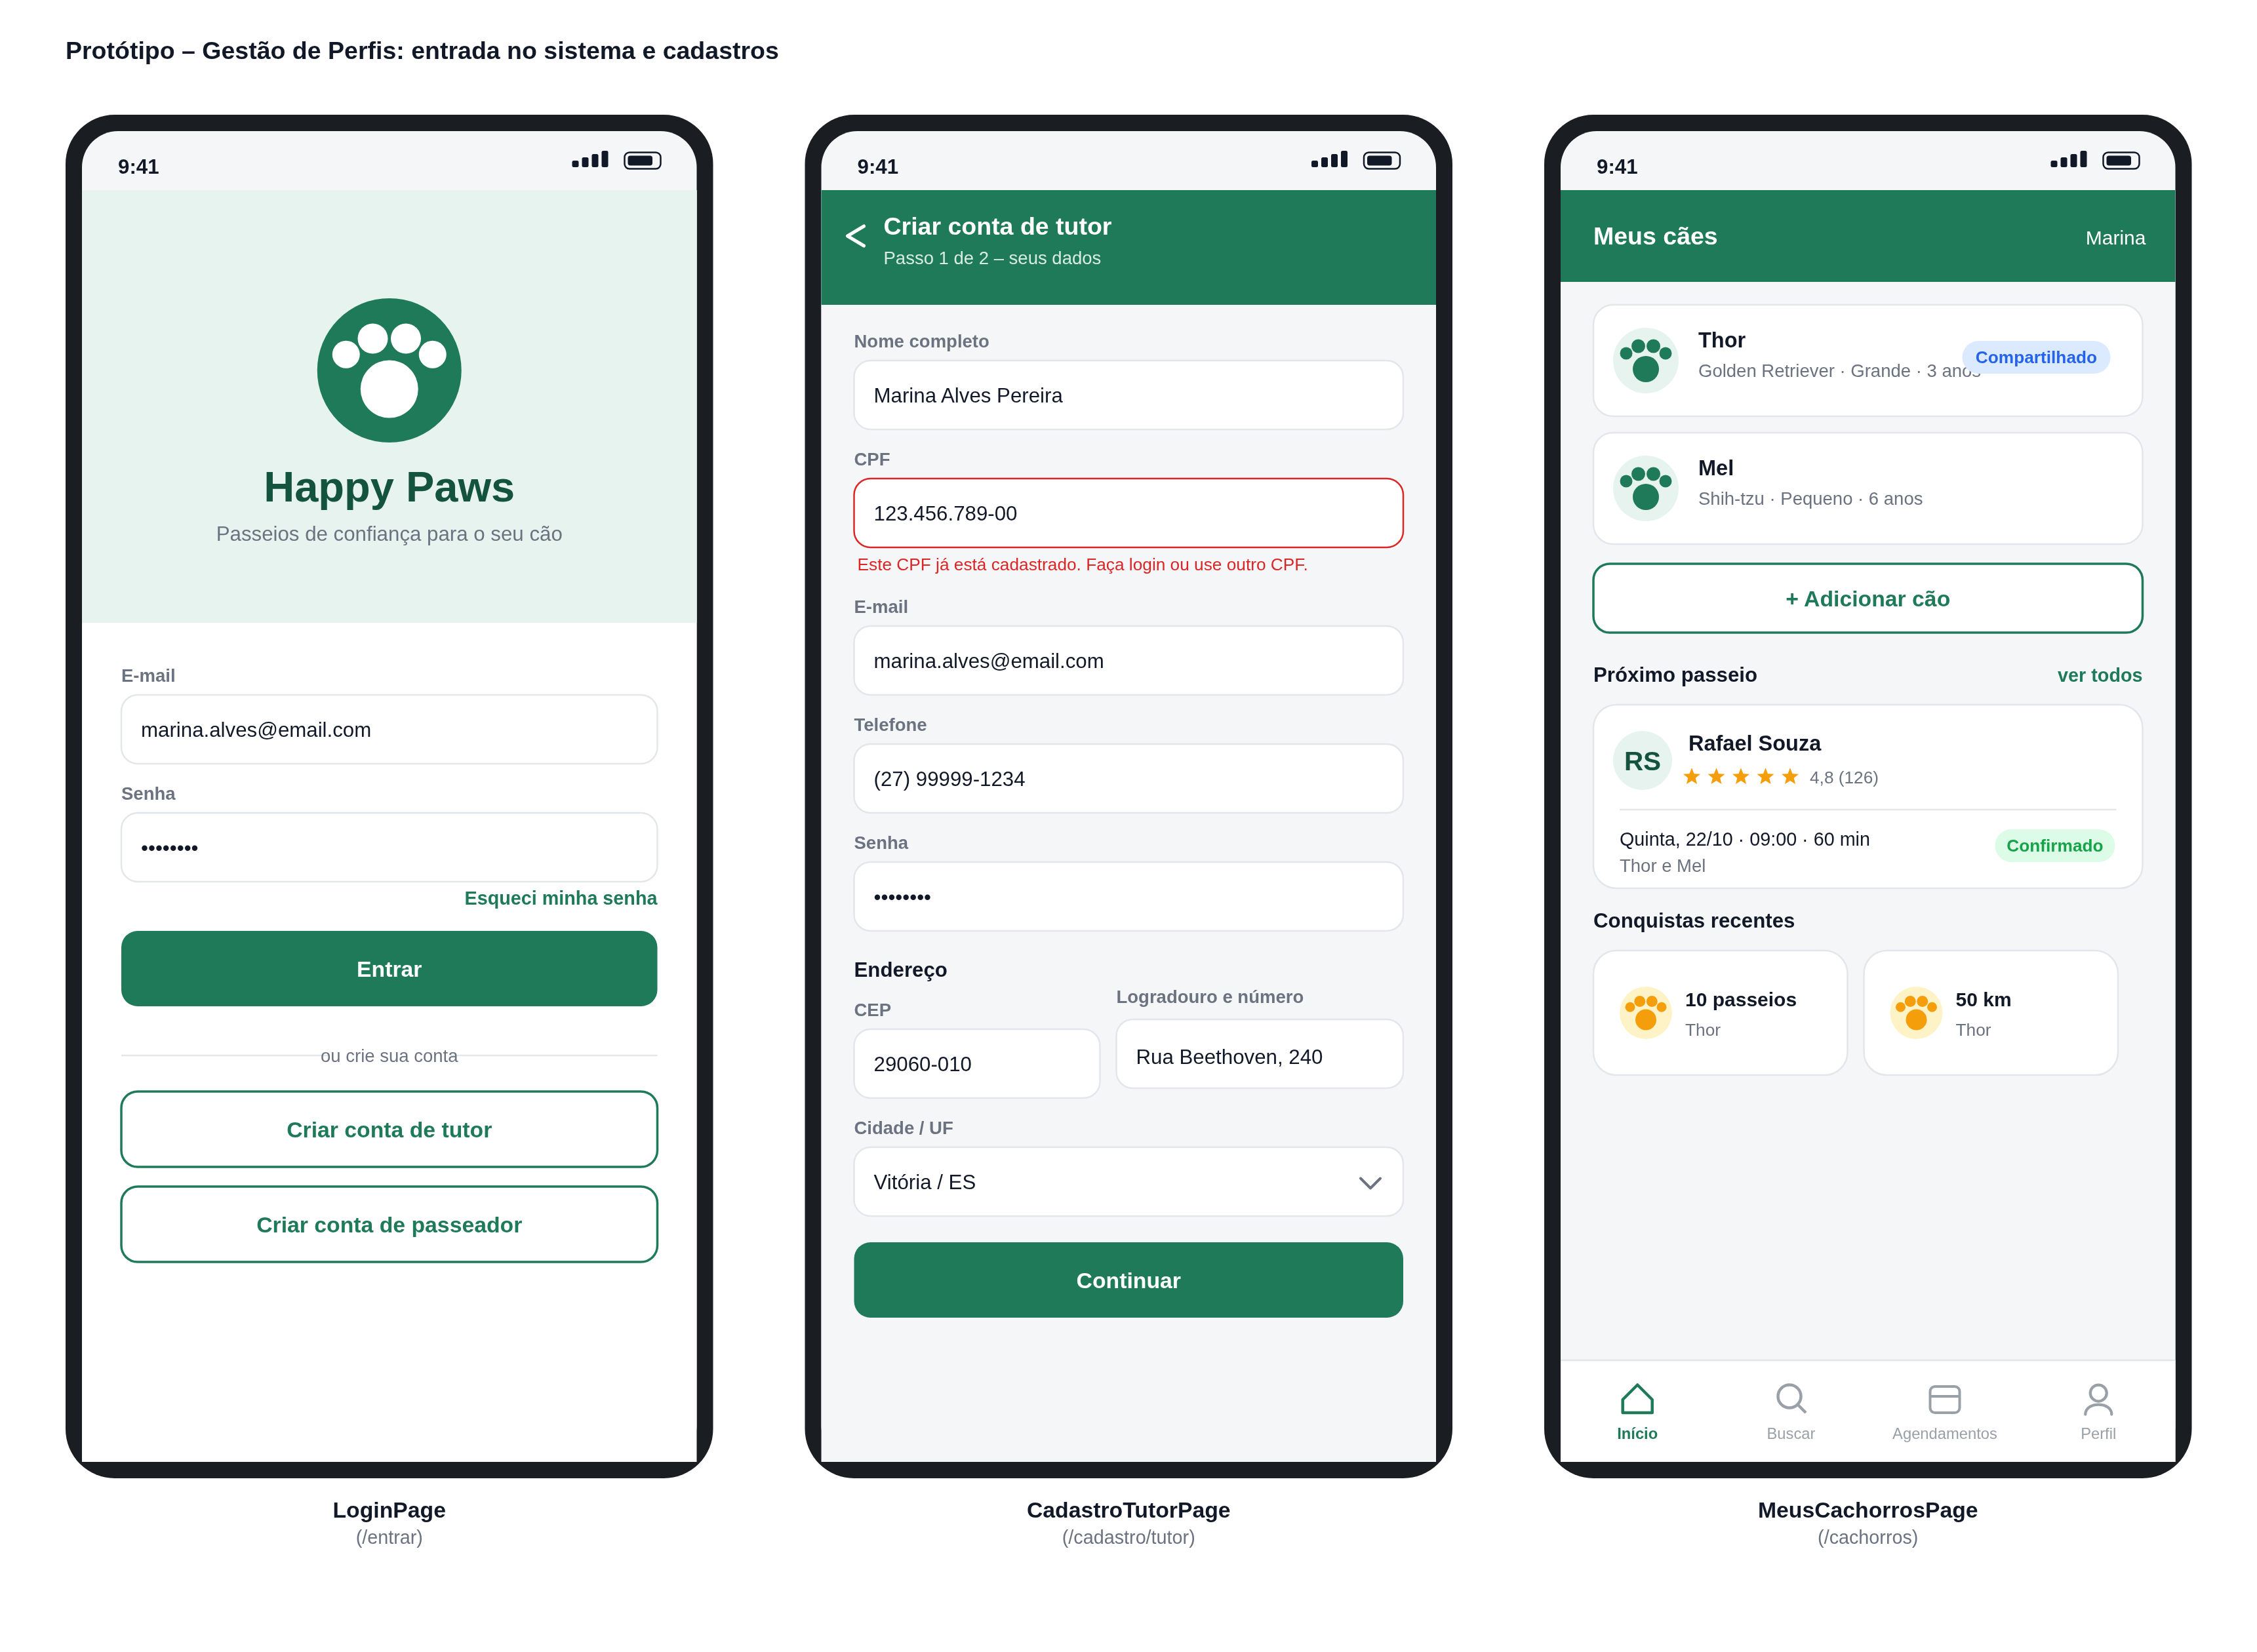
\includegraphics[width=1\textwidth,height=0.85\textheight,keepaspectratio]{figuras/proto-folha-perfis-1.png}
	\caption{Protótipo do subsistema Gestão de Perfis: entrada no sistema e cadastros.}
	\label{figura-proto-perfis-1}
\end{figure}

\begin{figure}[htbp]
	\centering
	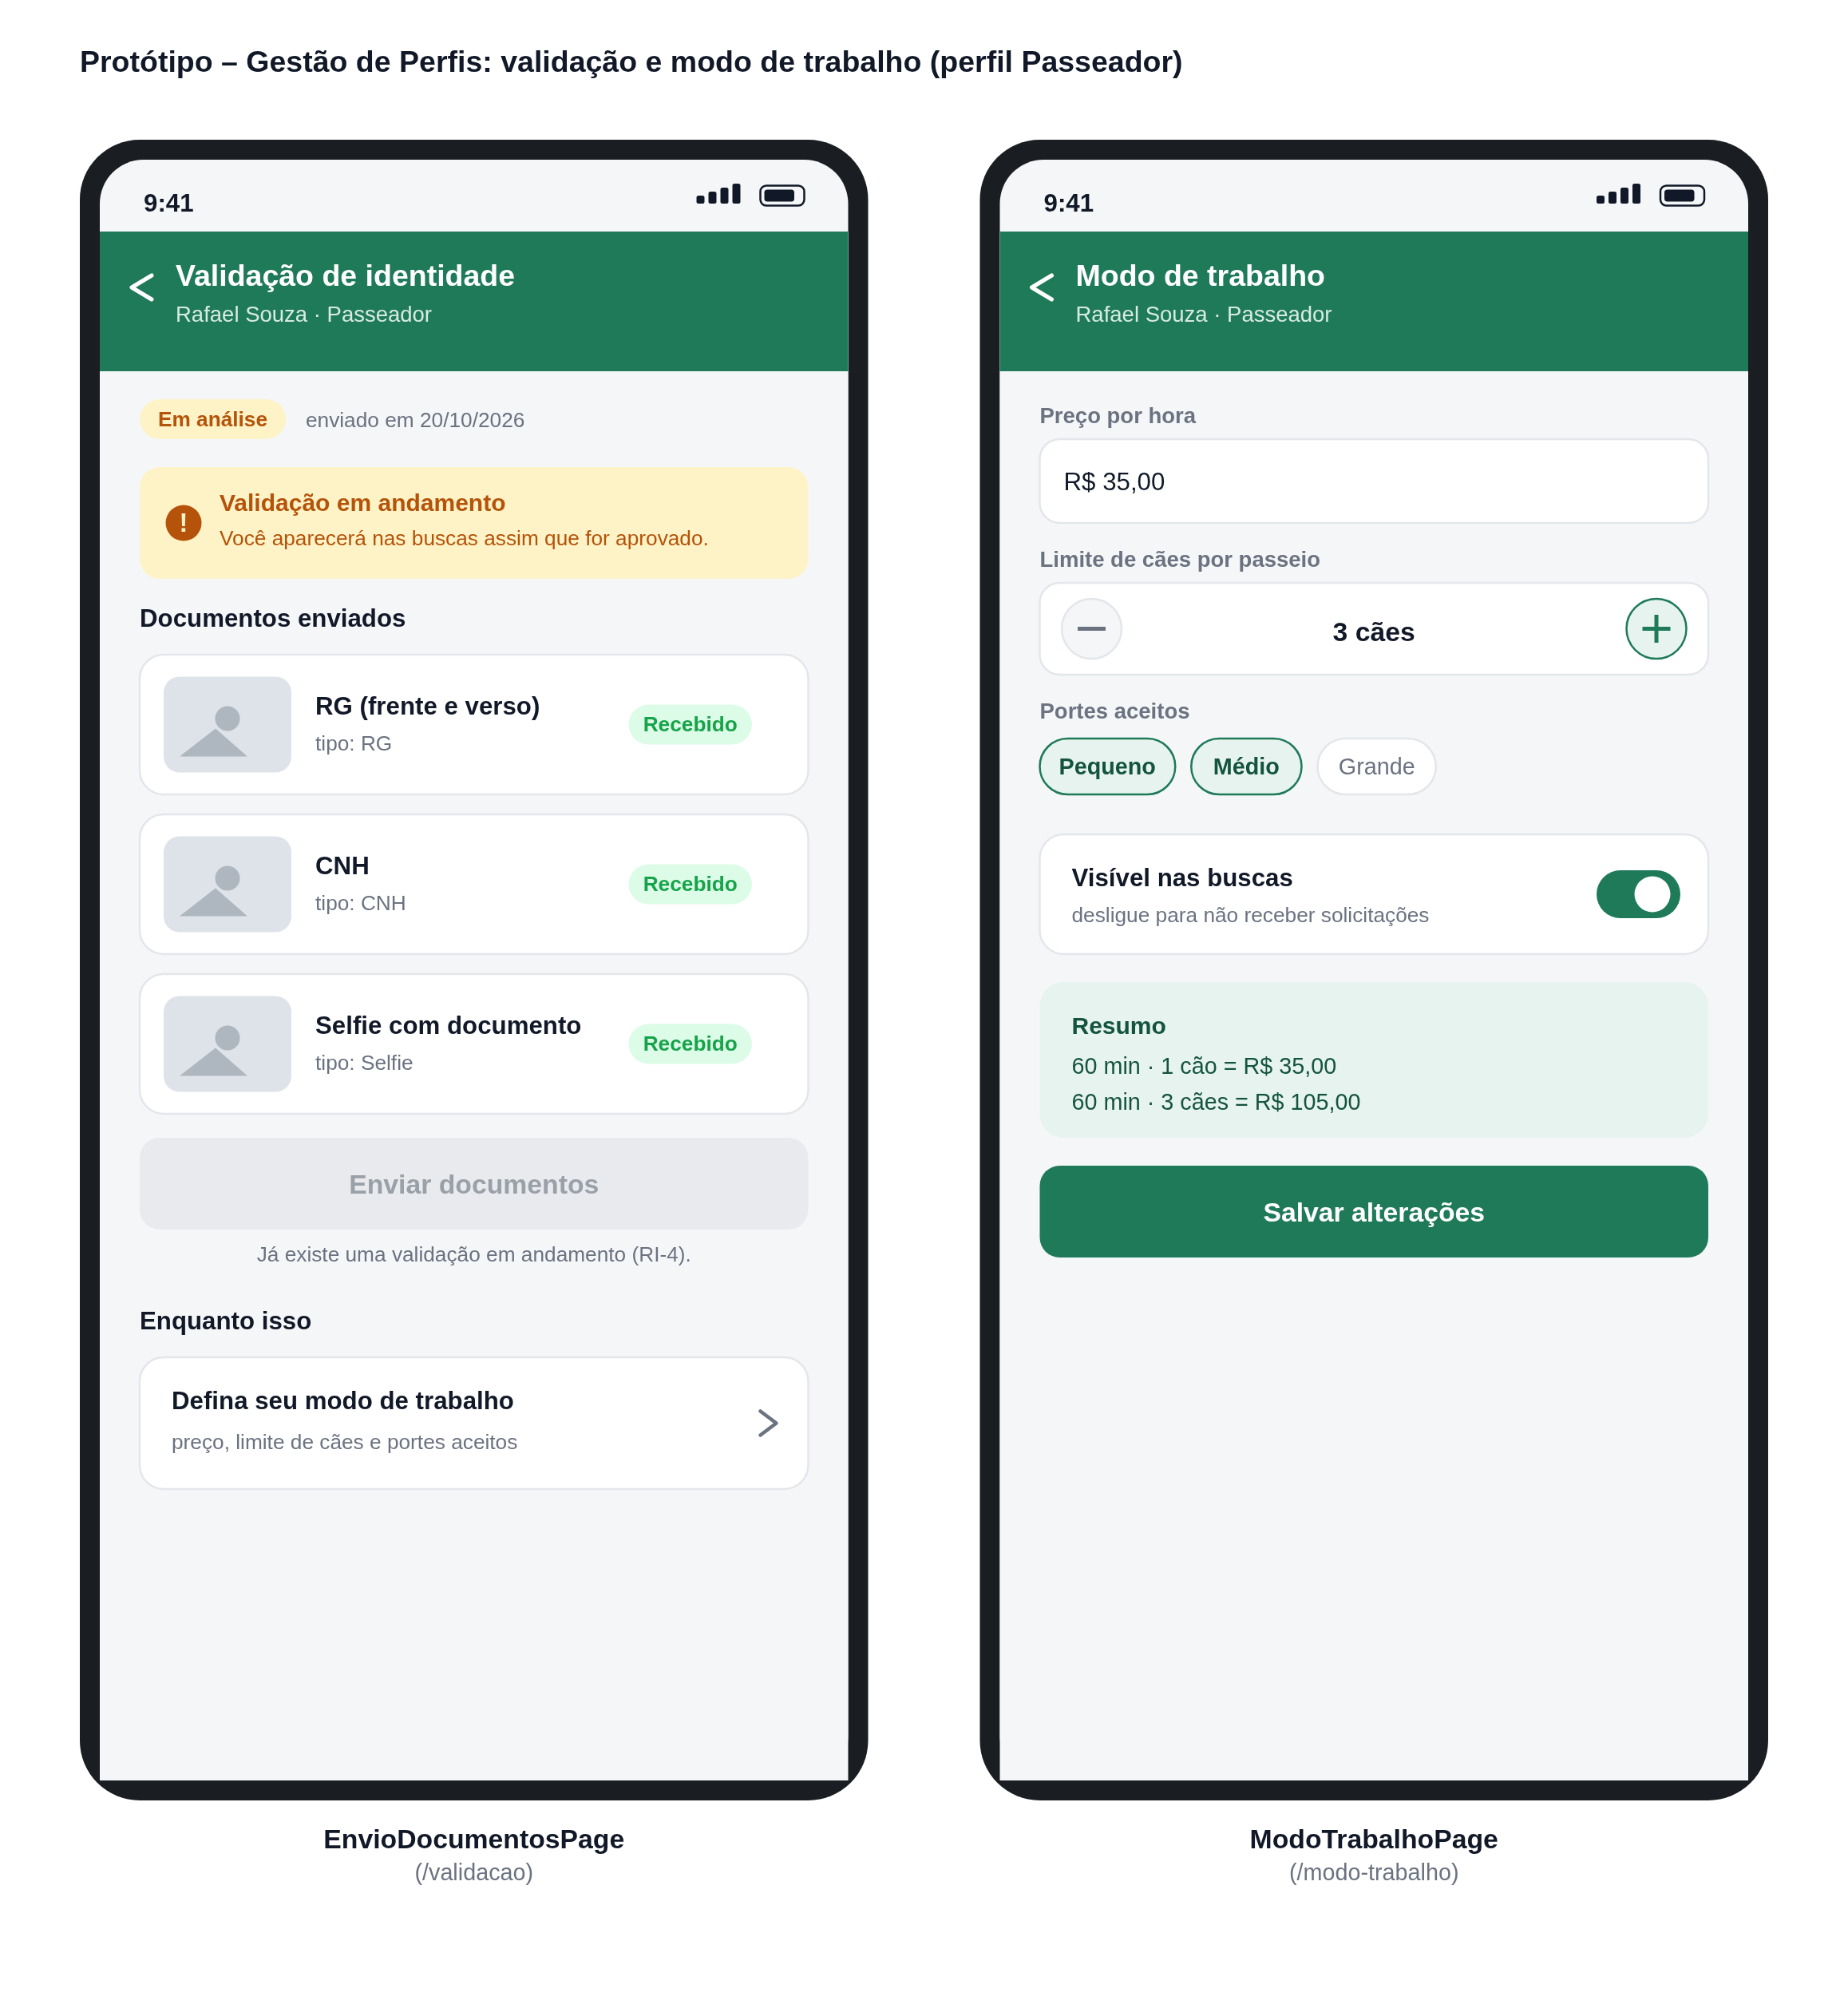
\includegraphics[width=0.68\textwidth,height=0.85\textheight,keepaspectratio]{figuras/proto-folha-perfis-2.png}
	\caption{Protótipo do subsistema Gestão de Perfis: validação de identidade e modo de trabalho (perfil Passeador).}
	\label{figura-proto-perfis-2}
\end{figure}

% ------------------------------------------------------------- Serviços
\begin{figure}[htbp]
	\centering
	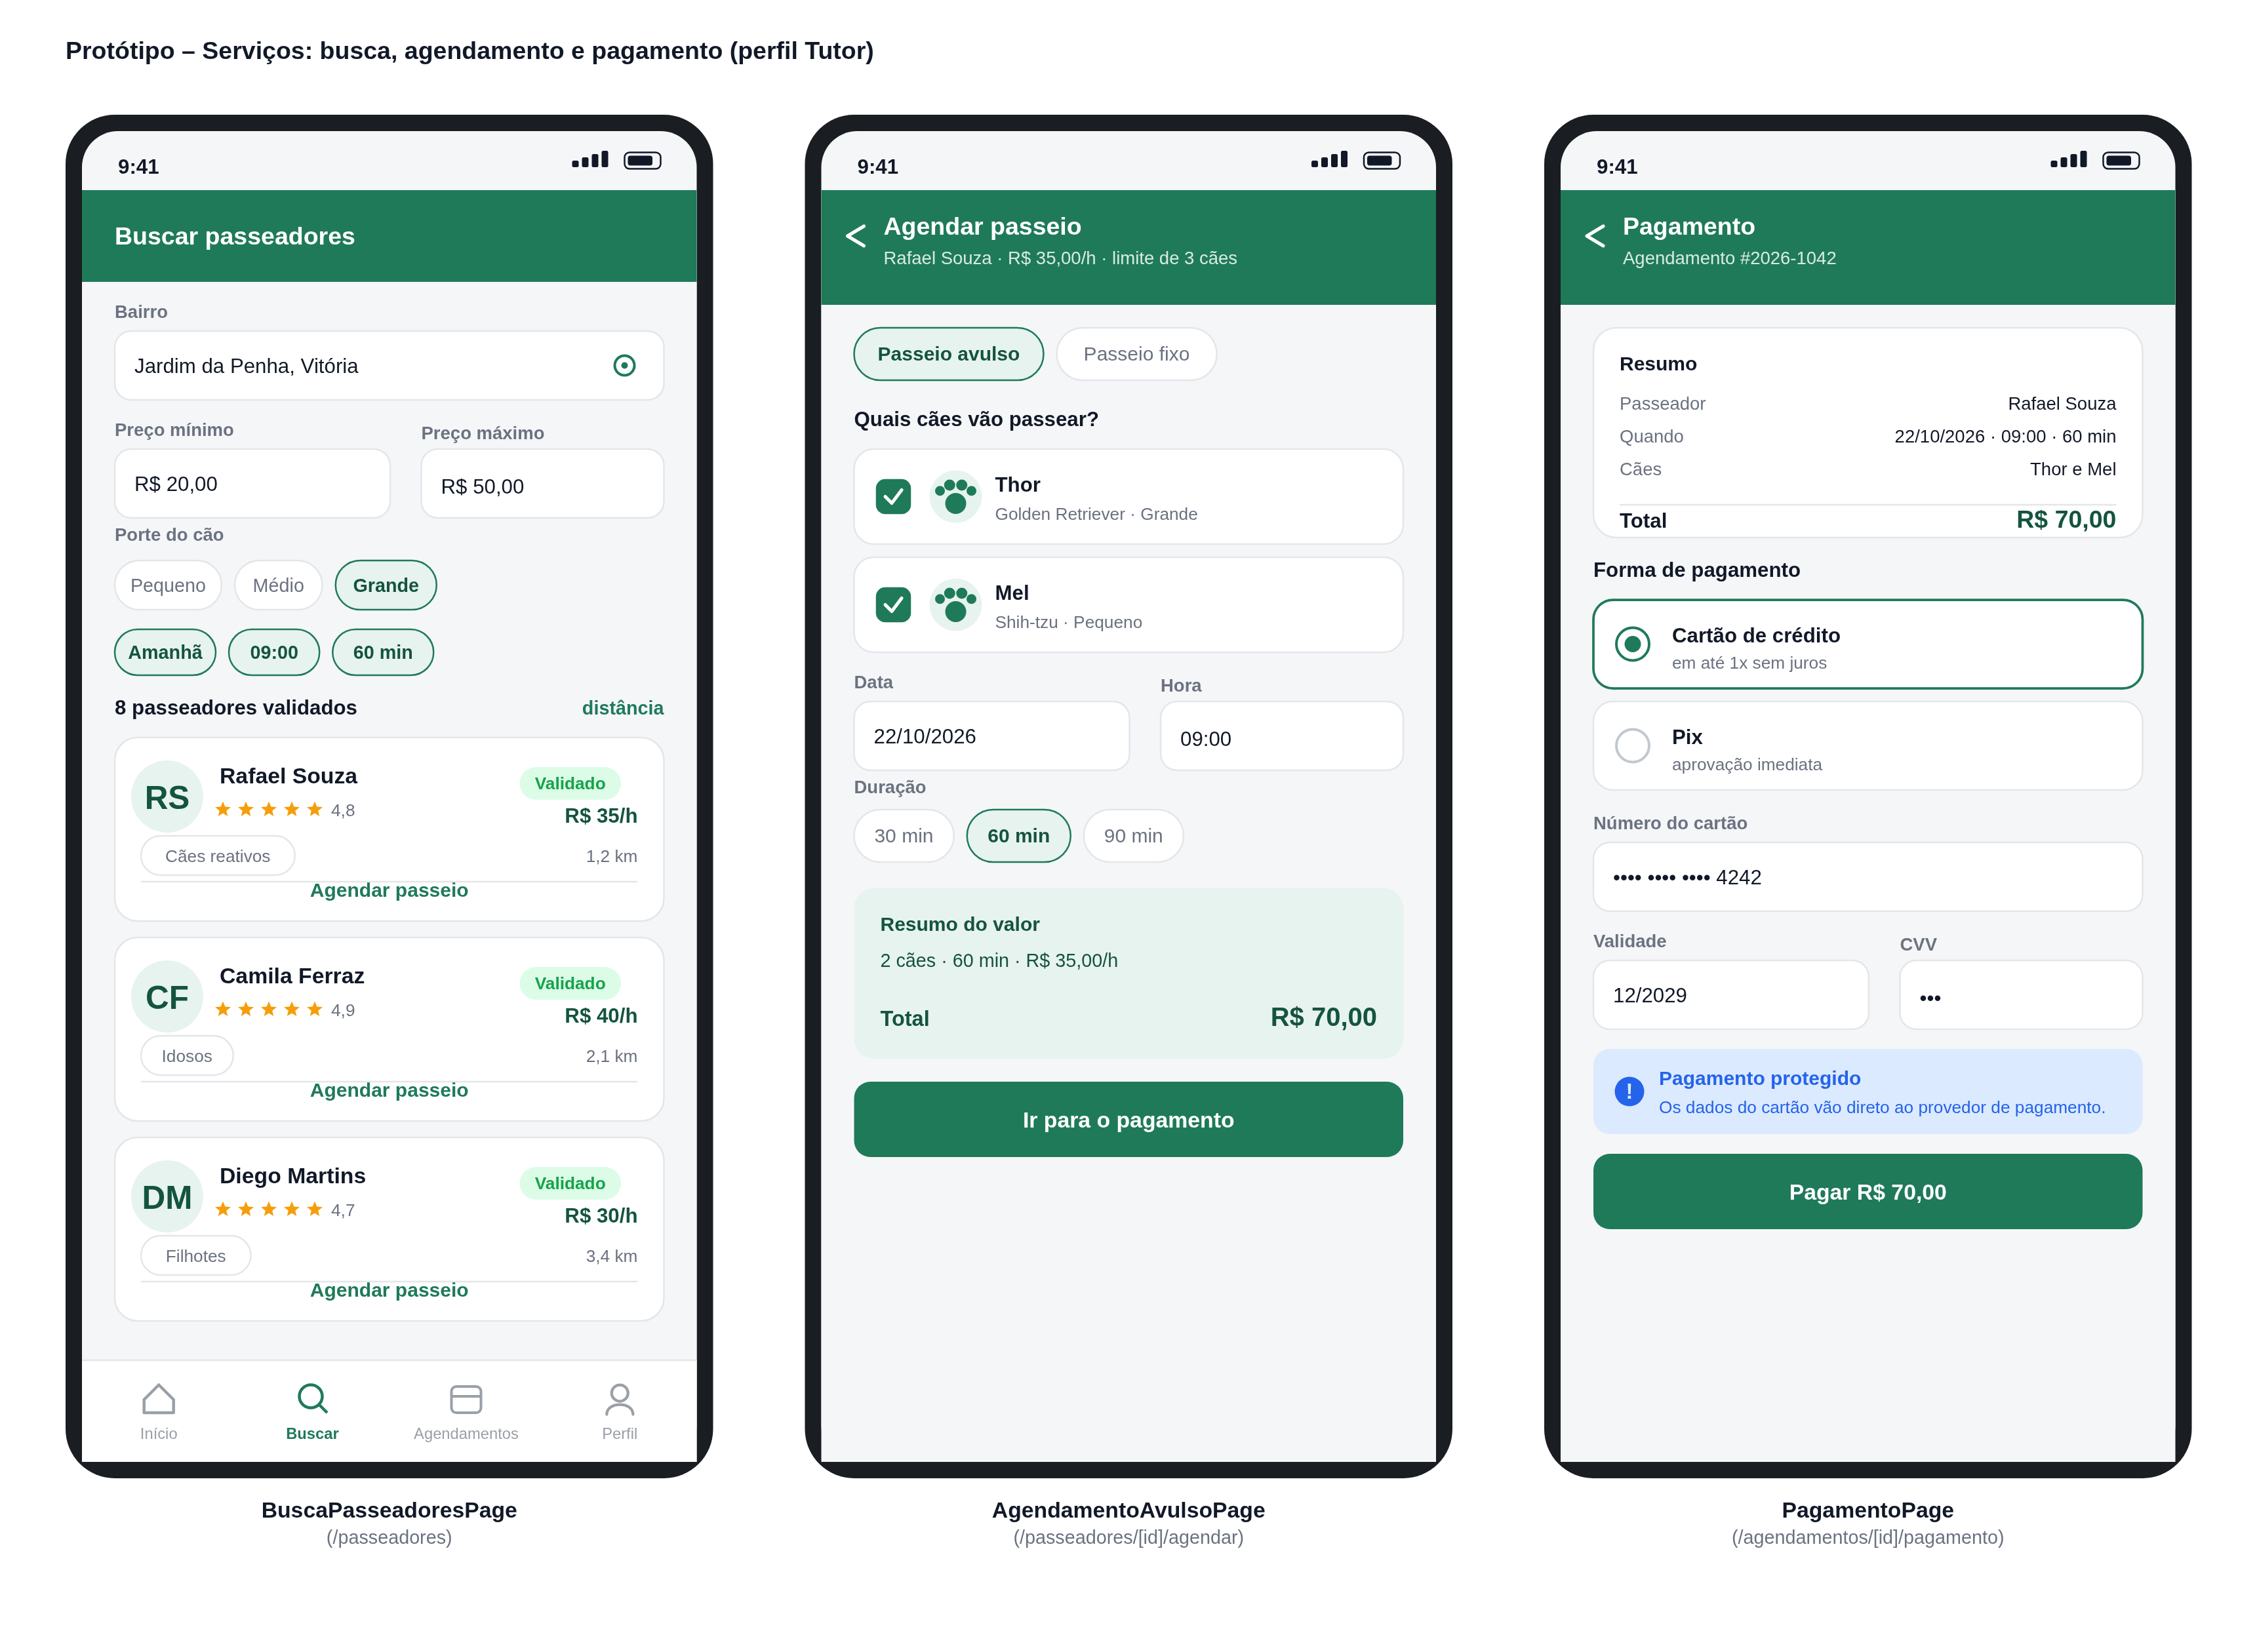
\includegraphics[width=1\textwidth,height=0.85\textheight,keepaspectratio]{figuras/proto-folha-servicos-1.png}
	\caption{Protótipo do subsistema Serviços: busca de passeadores, agendamento e pagamento (perfil Tutor).}
	\label{figura-proto-servicos-1}
\end{figure}

\begin{figure}[htbp]
	\centering
	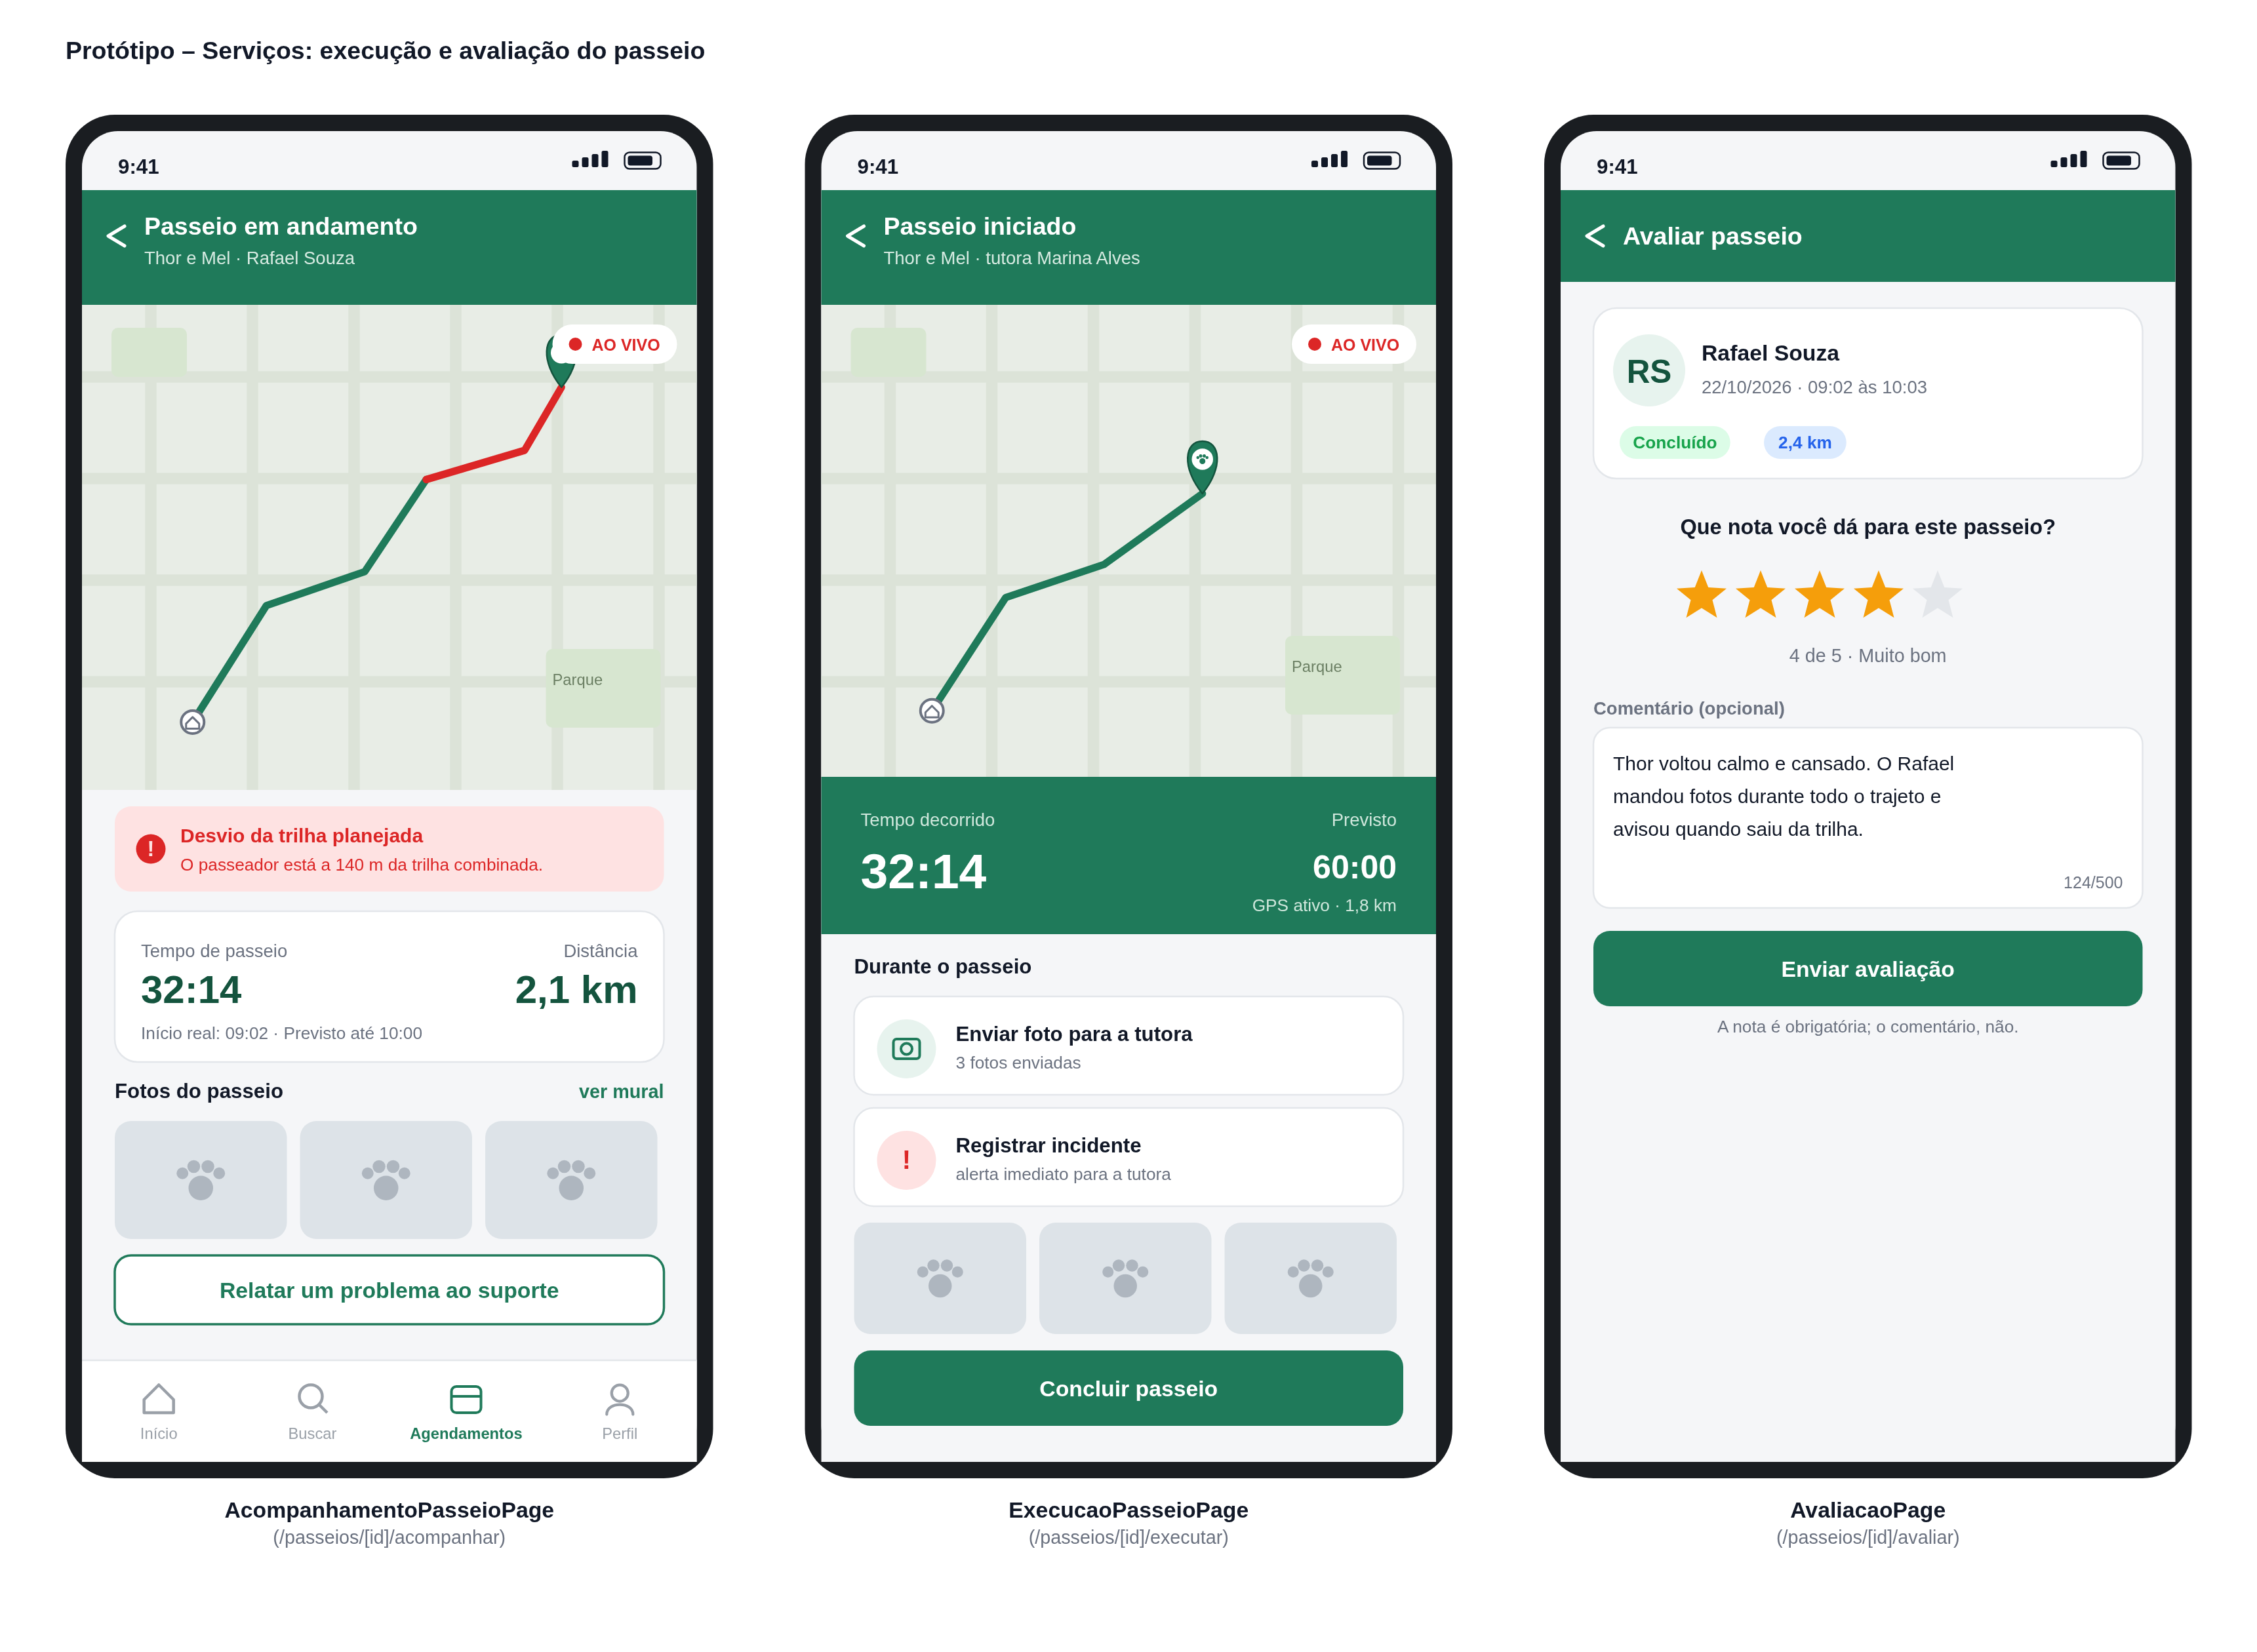
\includegraphics[width=1\textwidth,height=0.85\textheight,keepaspectratio]{figuras/proto-folha-servicos-2.png}
	\caption{Protótipo do subsistema Serviços: acompanhamento em tempo real, execução do passeio e avaliação.}
	\label{figura-proto-servicos-2}
\end{figure}

% -------------------------------------------------------------- Suporte
\begin{figure}[htbp]
	\centering
	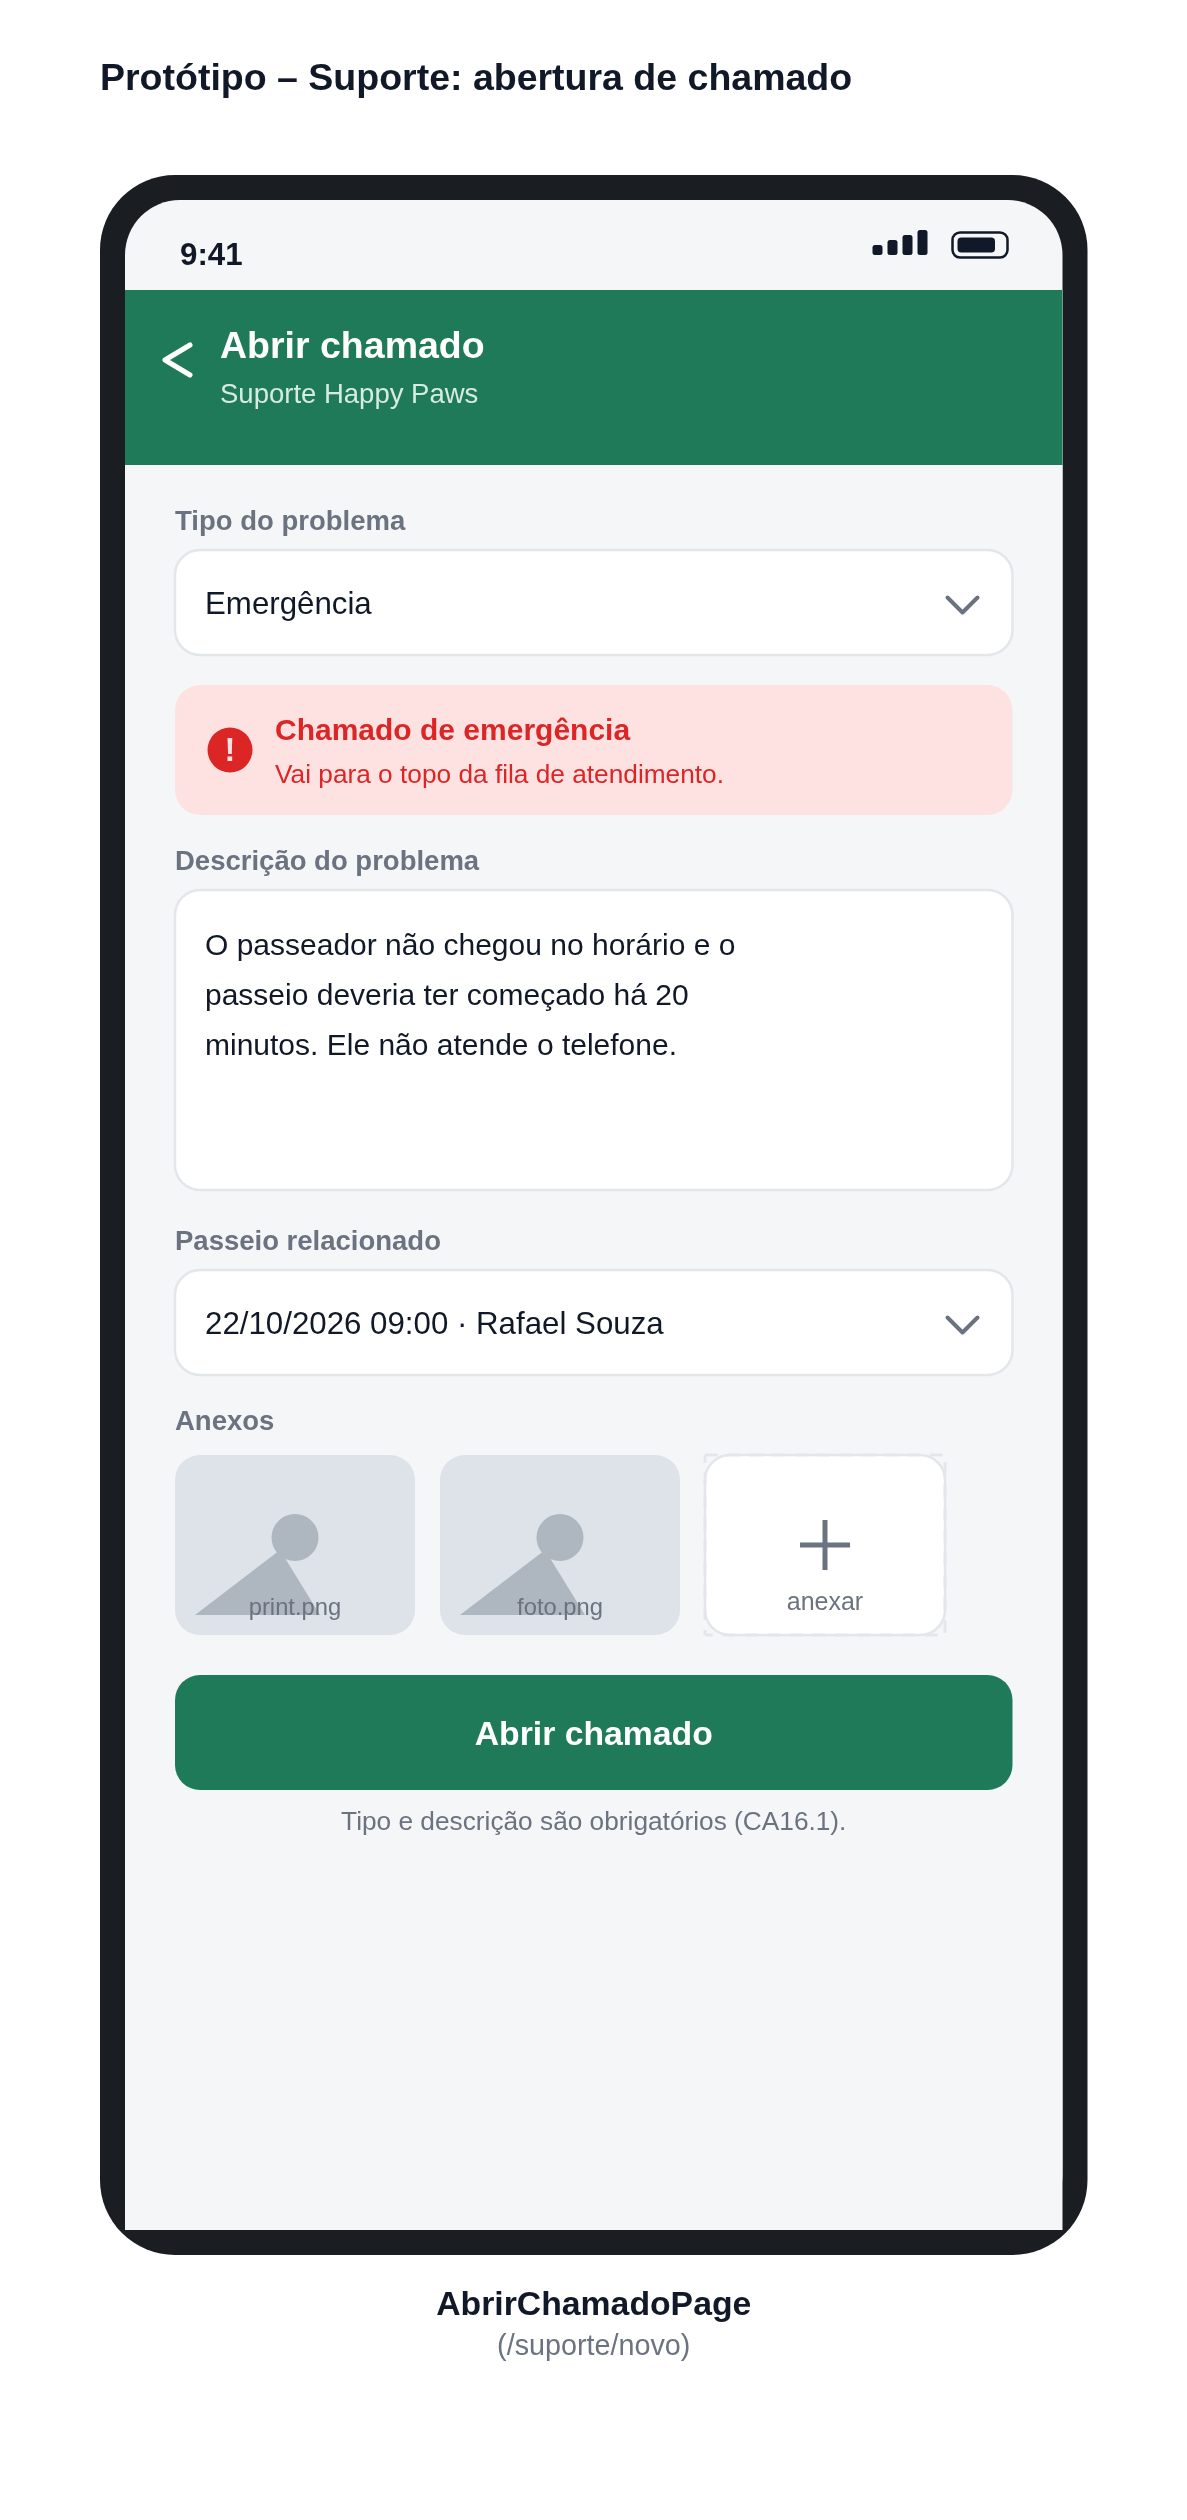
\includegraphics[width=0.29\textwidth,height=0.85\textheight,keepaspectratio]{figuras/proto-folha-suporte.png}
	\caption{Protótipo do subsistema Suporte: abertura de chamado pelo Tutor ou pelo Passeador.}
	\label{figura-proto-suporte}
\end{figure}

\begin{figure}[htbp]
	\centering
	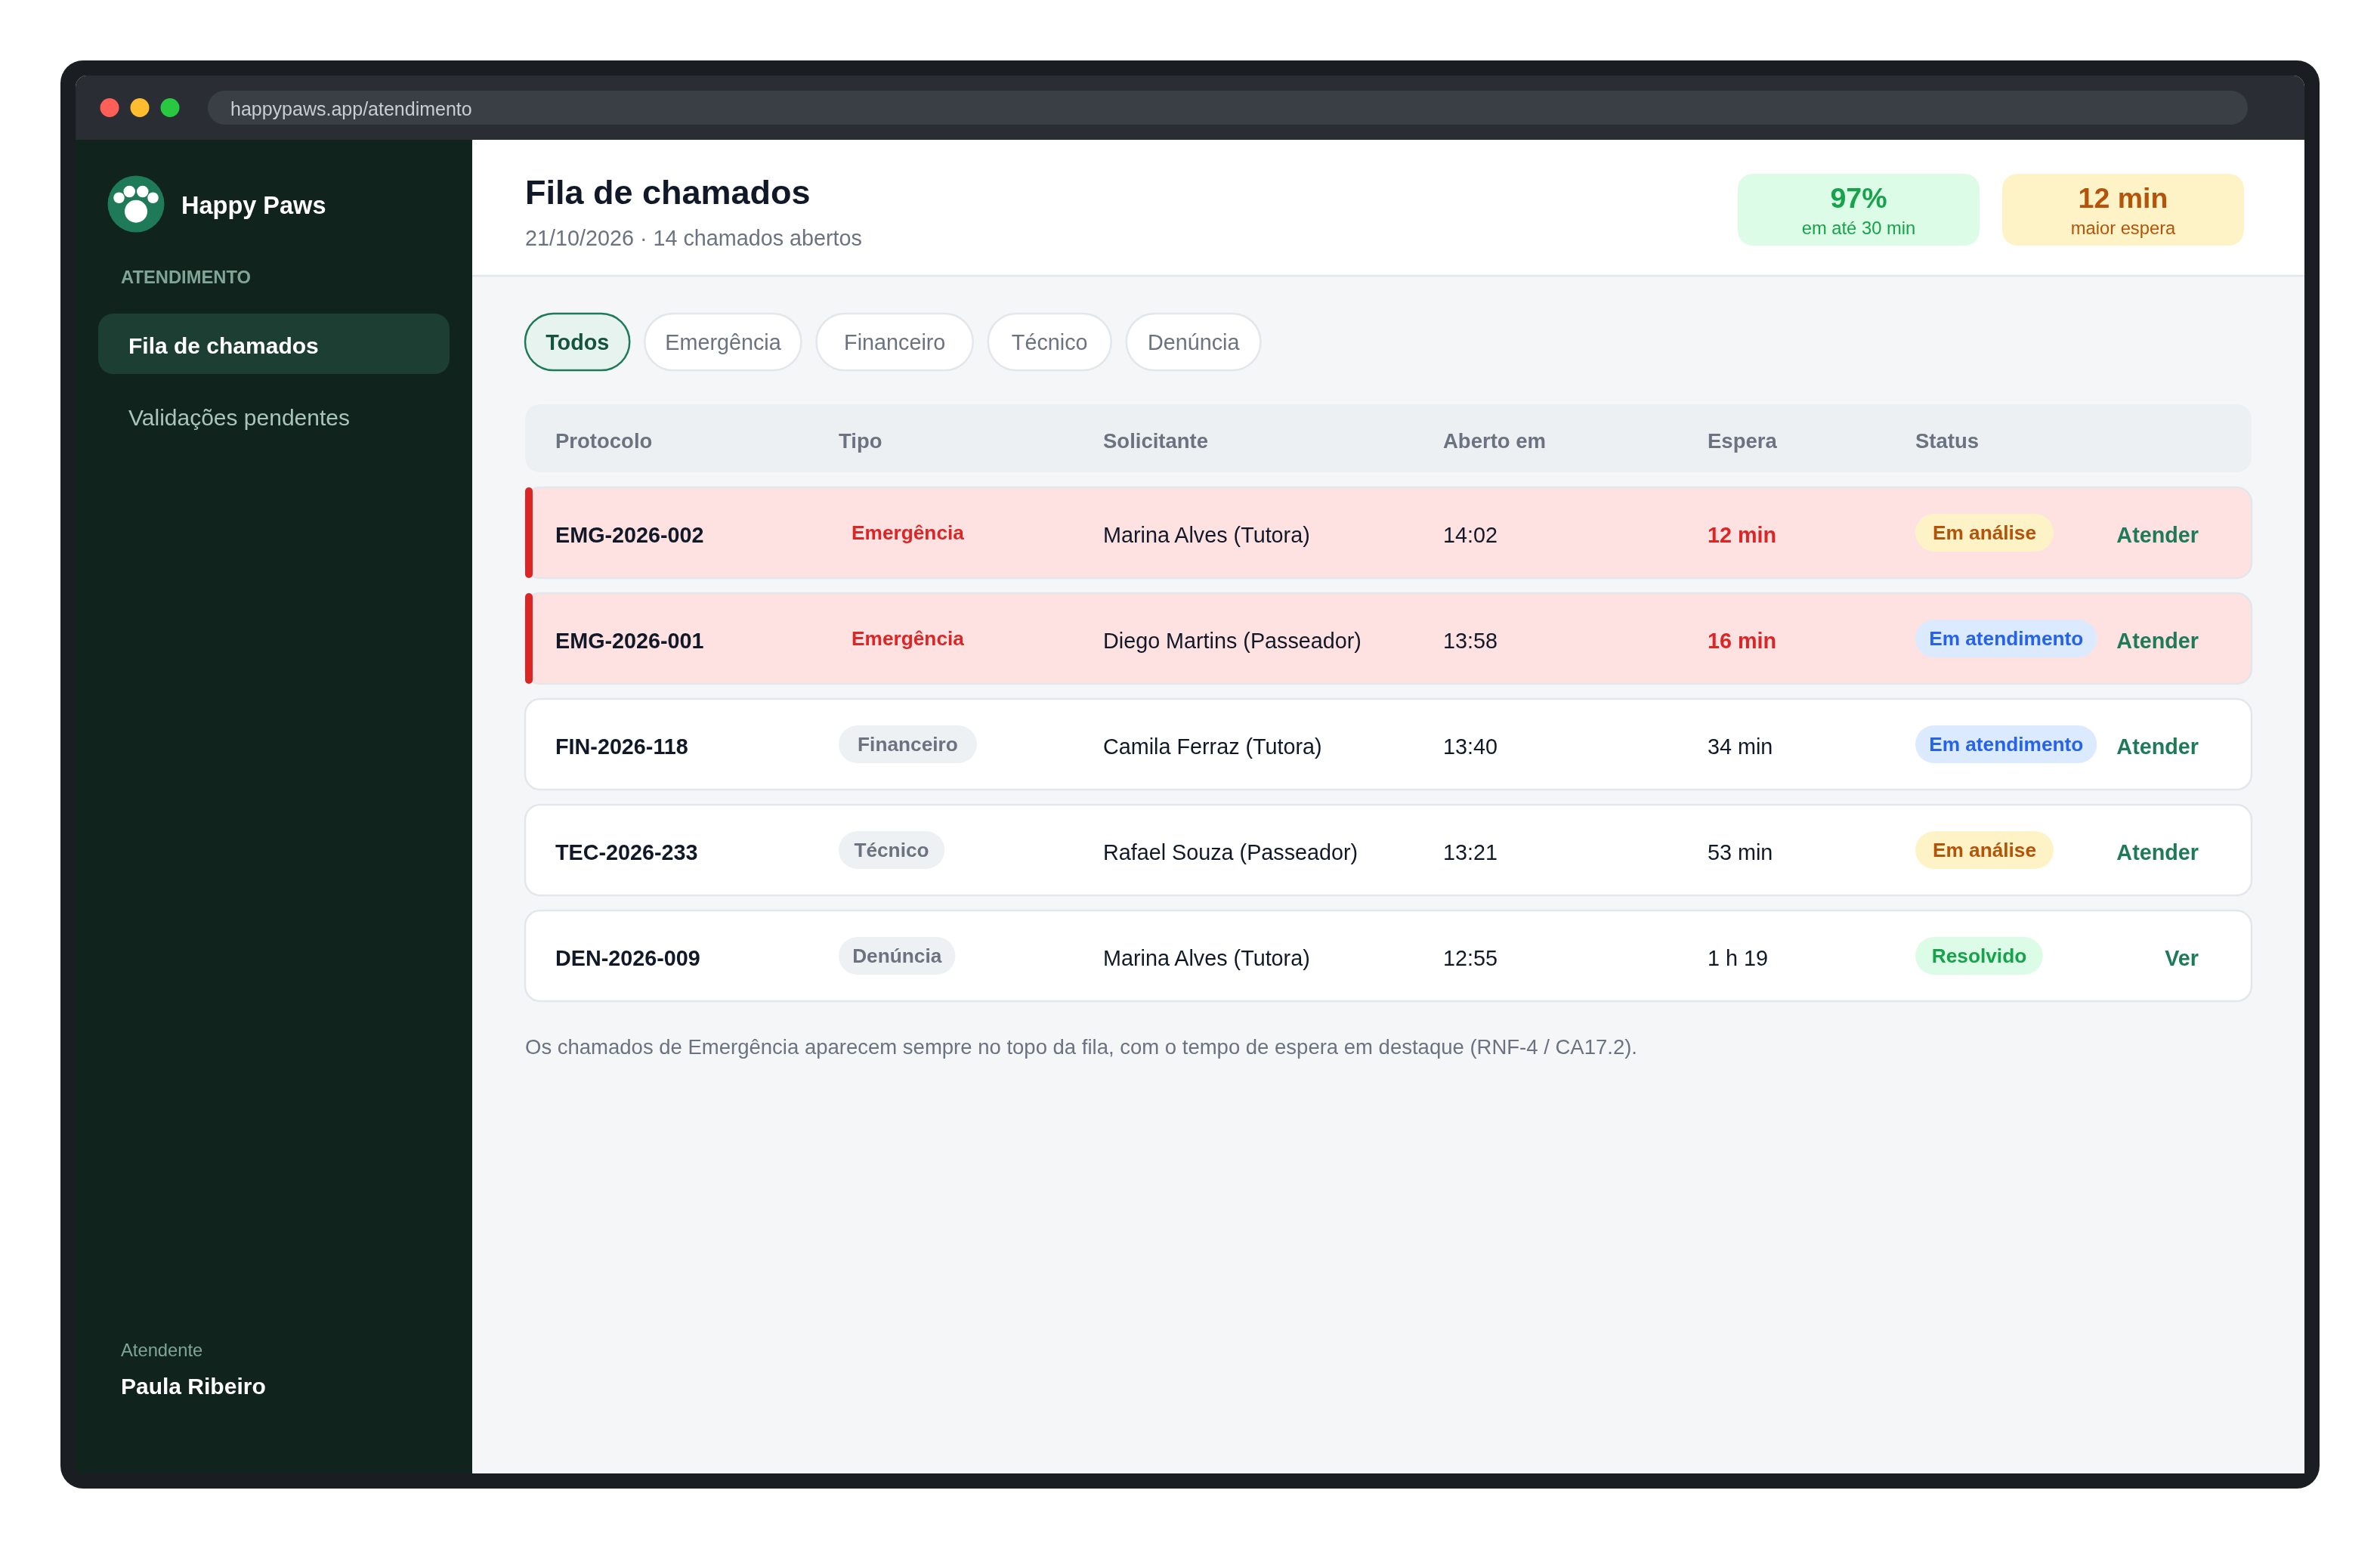
\includegraphics[width=1\textwidth,height=0.85\textheight,keepaspectratio]{figuras/proto-tela-13-fila-atendimento.png}
	\caption{Protótipo da central de atendimento (perfil Atendente): fila de chamados.}
	\label{figura-proto-fila}
\end{figure}

\begin{figure}[htbp]
	\centering
	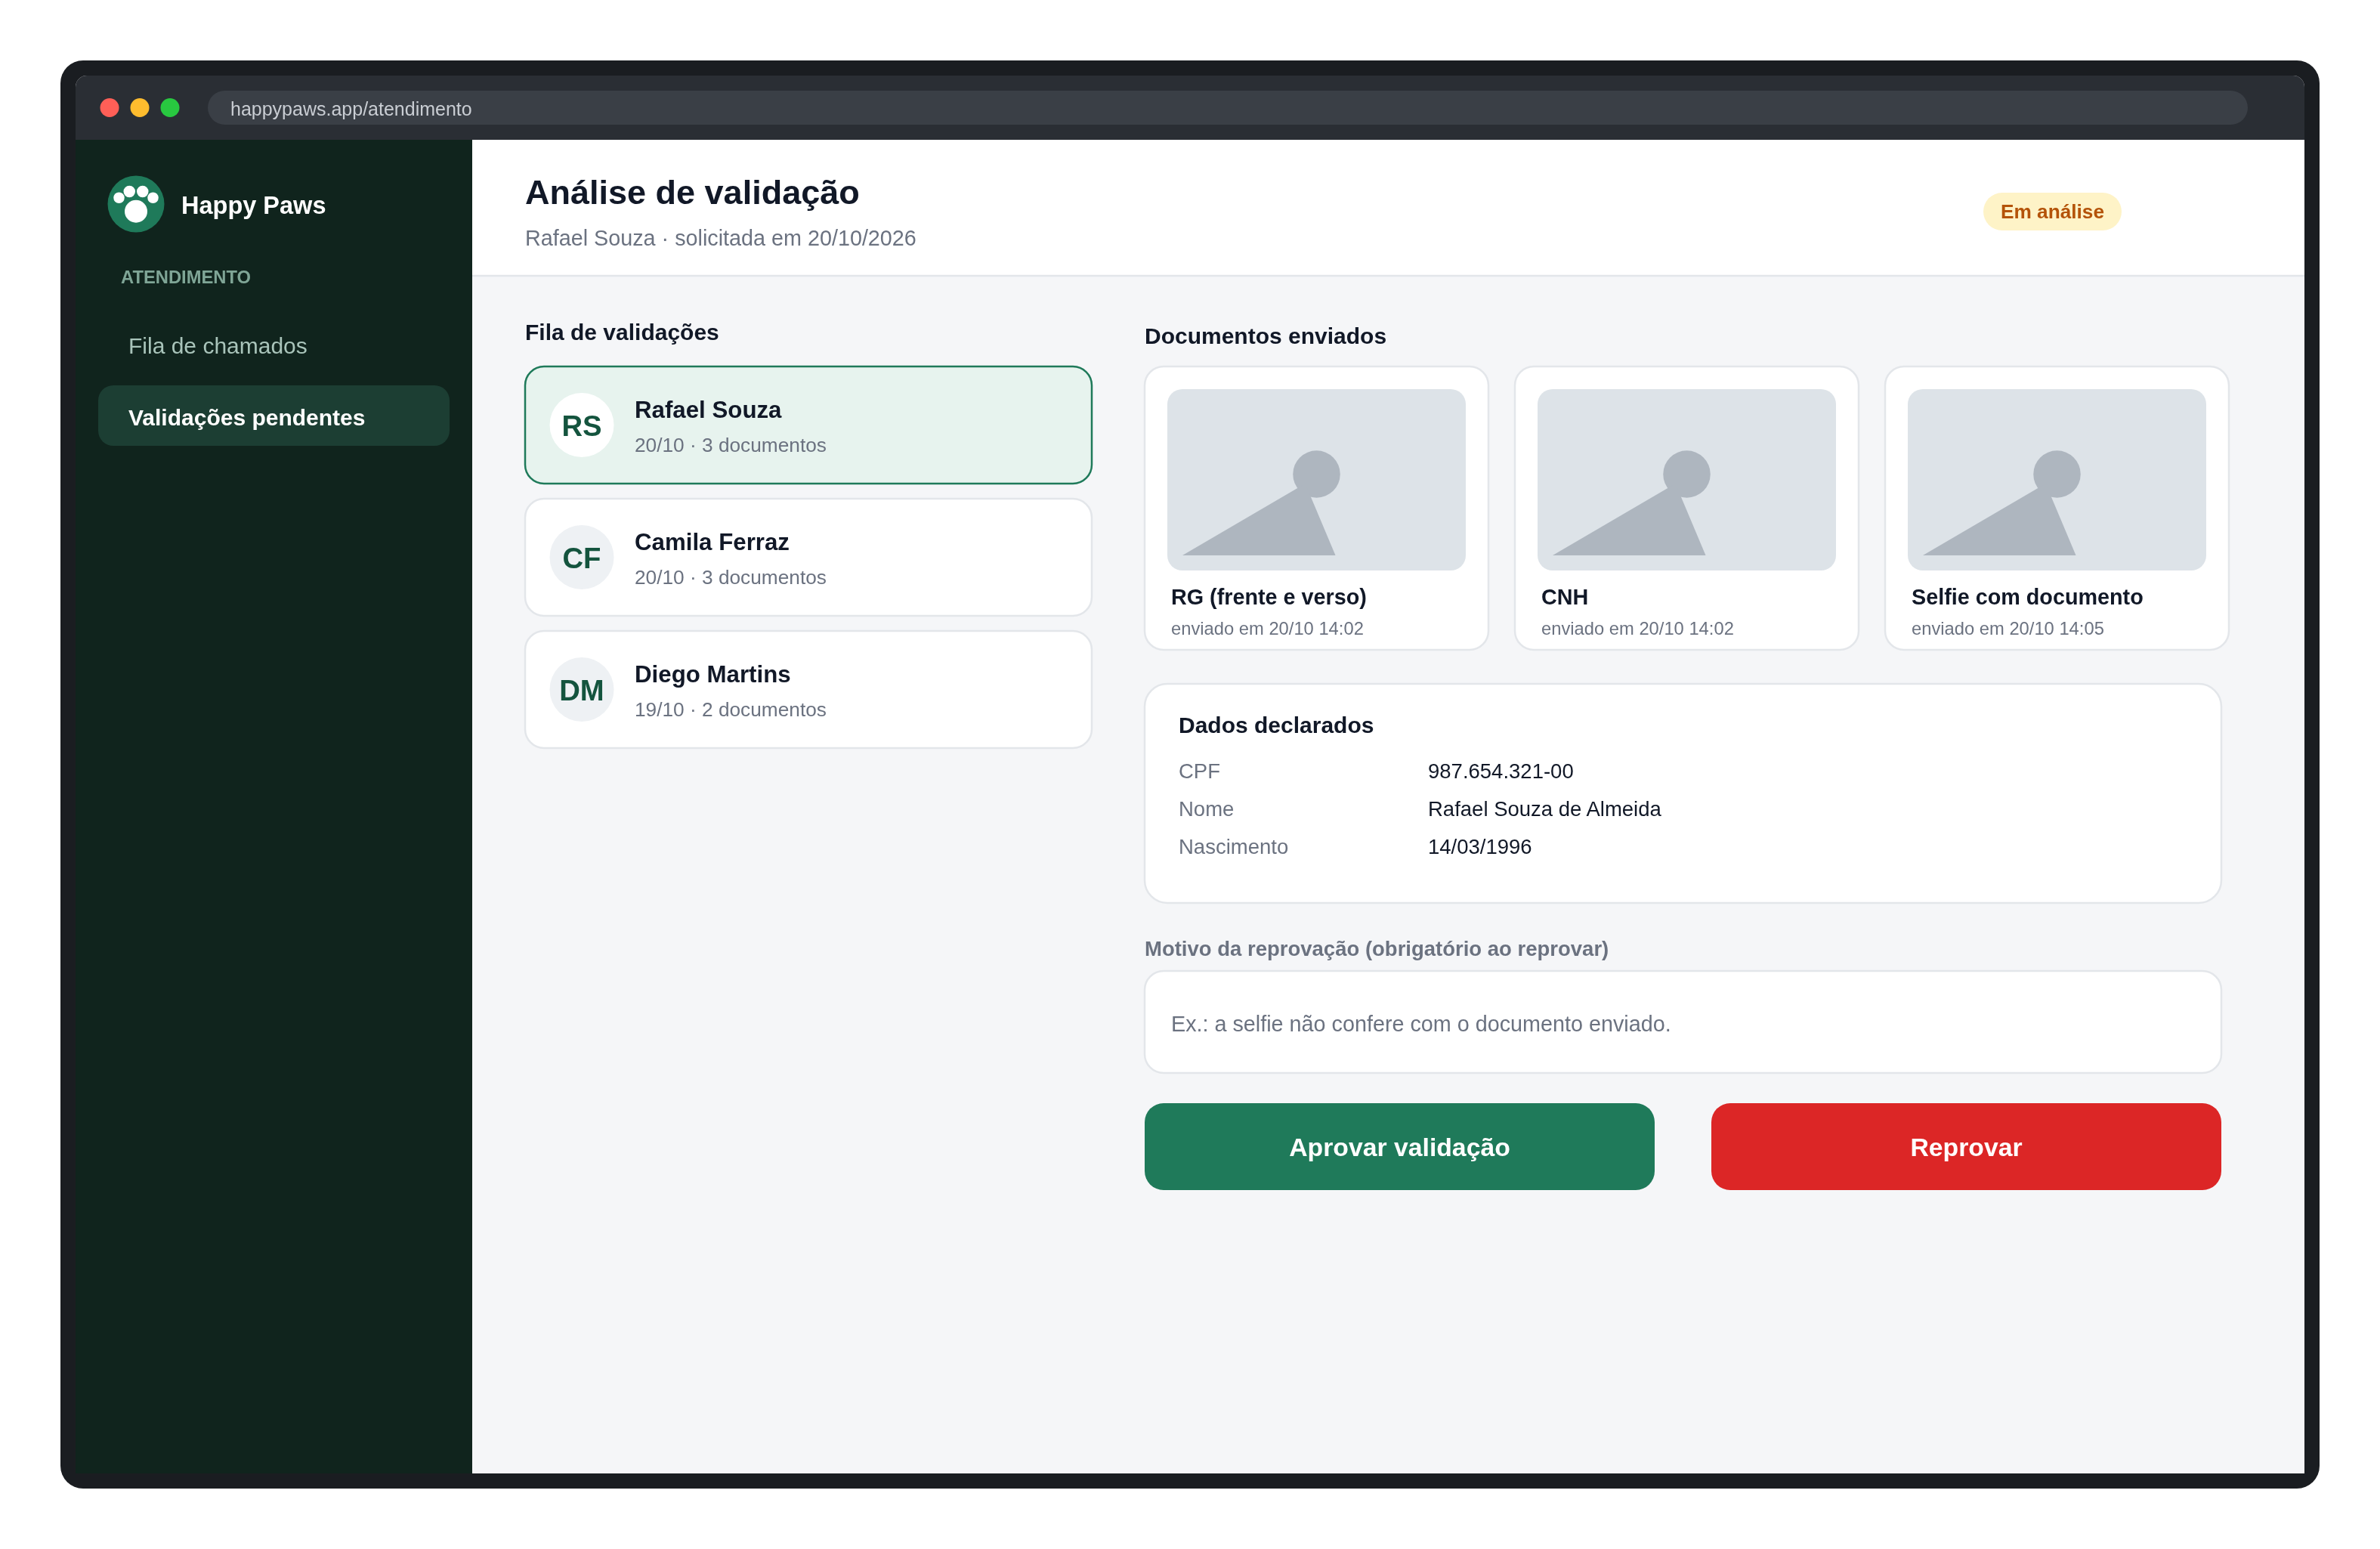
\includegraphics[width=1\textwidth,height=0.85\textheight,keepaspectratio]{figuras/proto-tela-14-analise-validacao.png}
	\caption{Protótipo da central de atendimento (perfil Atendente): análise de validação de identidade do Passeador.}
	\label{figura-proto-validacao}
\end{figure}

As decisões de projeto da interface registradas no protótipo são as seguintes:

\begin{sloppypar}
\begin{itemize}
	\item \textbf{Mensagens de erro junto ao campo.} Em \texttt{CadastroTutorPage} (Figura~\ref{figura-proto-perfis-1}), o erro de CPF já cadastrado (RI-1) aparece abaixo do próprio campo, em linguagem do usuário e com a ação sugerida, e não em uma mensagem genérica no topo da página;

	\item \textbf{Comandos inapropriados desabilitados.} Em \texttt{EnvioDocumentosPage} (Figura~\ref{figura-proto-perfis-2}), o botão de envio fica desabilitado enquanto houver uma validação em andamento (RI-4), e o motivo é informado logo abaixo do botão. A mesma tática vale para o botão ``Iniciar passeio'', que só é habilitado com o pagamento confirmado (CA14.5);

	\item \textbf{Entrada por seleção.} Porte, especialidades, portes aceitos, duração, tipo de agendamento, método de pagamento, tipo de documento e tipo de chamado são escolhidos em listas, botões de opção ou \textit{chips}, nunca digitados (Tabela~\ref{tabela-enumerados}); a localização da busca é obtida pela \textit{Geolocation API} e os cães do agendamento vêm da lista de cães do próprio Tutor;

	\item \textbf{Resumo antes do compromisso.} As telas de agendamento e de pagamento (Figura~\ref{figura-proto-servicos-1}) mostram o valor calculado por \texttt{Agendamento.calcularValor()} antes de o Tutor confirmar, e a tela de pagamento informa que os dados do cartão são enviados diretamente ao provedor de pagamento (RNF-2);

	\item \textbf{Estado do sistema sempre visível.} A tela de acompanhamento (Figura~\ref{figura-proto-servicos-2}) tem o indicador ``AO VIVO'', o tempo decorrido, a distância percorrida e o aviso de desvio de rota em destaque; o trecho fora da trilha planejada aparece em vermelho no mapa (CA10.3);

	\item \textbf{Telas de uso em movimento.} A tela de execução do passeio (perfil Passeador) usa poucos comandos, botões grandes, alto contraste e nenhuma digitação obrigatória: o cronômetro e os comandos de foto, de incidente e de conclusão ocupam toda a largura da tela;

	\item \textbf{Iniciativa do sistema na fila de atendimento.} Em \texttt{FilaAtendimentoPage} (Figura~\ref{figura-proto-fila}), os chamados do tipo ``Emergência'' aparecem no topo, com faixa e tempo de espera em destaque, e o indicador de primeiro atendimento em até 30 minutos fica no cabeçalho (RNF-4 e CA17.2);

	\item \textbf{Dados obrigatórios no momento certo.} Na análise de validação (Figura~\ref{figura-proto-validacao}), o campo de motivo fica junto dos botões e é obrigatório apenas quando o Atendente reprova a validação (CA04.4); na avaliação do passeio, a nota é obrigatória e o comentário é opcional.
\end{itemize}
\end{sloppypar}

Em relação ao protótipo de Engenharia de Software I, esta versão acrescenta as telas do perfil Atendente (fila de chamados e análise de validação), separa as páginas por rota e por perfil, conforme as Tabelas~\ref{tabela-ciu-perfis} a~\ref{tabela-ciu-suporte}, e incorpora as táticas de usabilidade da Tabela~\ref{tabela-taticas-usabilidade}.

O protótipo completo desta revisão pode ser visto na Web em \url{https://raw.githack.com/Eduardo-Ferraz/happy-paws-go/main/docs/es2-projeto/prototipo/index.html}. Os arquivos ficam no repositório do projeto, em \url{https://github.com/Eduardo-Ferraz/happy-paws-go/tree/main/docs/es2-projeto/prototipo}, em formato vetorial (SVG), uma tela por arquivo, nomeadas pela página correspondente do pacote \texttt{cih}.



%=======================================================================================================
\FloatBarrier
\section{Subsistema Gestão de Perfis}
\label{sec-ihc-perfis}

A Figura~\ref{figura-ciu-perfis} mostra o projeto da Camada de Interface com o Usuário (pacotes \texttt{cih} e \texttt{cci}) do subsistema Gestão de Perfis, juntamente com as classes de aplicação do pacote \texttt{cgt} das quais os controladores dependem (Figura~\ref{figura-ln-perfis-cgt}). As telas correspondem às Figuras 1 a 7 do documento de requisitos. A Tabela~\ref{tabela-ciu-perfis} lista as páginas, suas rotas, os perfis que as acessam e os controladores responsáveis.

\begin{figure}[h]
	\centering
	\figciu{figuras/ciu-perfis.png}{0.85}
	\caption{Projeto da Camada de Interface com o Usuário (\texttt{cih} e \texttt{cci}) do subsistema Gestão de Perfis.}
	\label{figura-ciu-perfis}
\end{figure}

\begin{scriptsize}
\setlength{\tabcolsep}{3pt}
\begin{longtable}{|p{4.2cm}|p{3.6cm}|p{1.7cm}|p{1.3cm}|p{3.8cm}|}
	\caption{Páginas do subsistema Gestão de Perfis.}
	\label{tabela-ciu-perfis}\\\hline
	\rowcolor{lightgray}
	\textbf{Página} & \textbf{Rota} & \textbf{Perfil} & \textbf{US} & \textbf{Controlador} \\\hline
	\endfirsthead
	\hline
	\rowcolor{lightgray}
	\textbf{Página} & \textbf{Rota} & \textbf{Perfil} & \textbf{US} & \textbf{Controlador} \\\hline
	\endhead
	\texttt{LoginPage} & \texttt{/entrar} & Todos & US01, US03 & \texttt{CadastroUsuario\-Controller} \\\hline
	\texttt{CadastroTutorPage} & \texttt{/cadastro/tutor} & Visitante & US01 & \texttt{CadastroUsuario\-Controller} \\\hline
	\texttt{CadastroPasseadorPage} & \texttt{/cadastro/\allowbreak passeador} & Visitante & US03 & \texttt{CadastroUsuario\-Controller} \\\hline
	\texttt{EditarPerfilPage} & \texttt{/perfil} & Tutor, Passeador & US01, US03 & \texttt{CadastroUsuario\-Controller} \\\hline
	\texttt{MeusCachorrosPage} & \texttt{/cachorros} & Tutor & US02 & \texttt{CadastroCachorro\-Controller} \\\hline
	\texttt{CadastroCachorroPage} & \texttt{/cachorros/novo} e \texttt{/cachorros/\allowbreak [id]/editar} & Tutor & US02 & \texttt{CadastroCachorro\-Controller} \\\hline
	\texttt{CompartilharPerfilPage} & \texttt{/cachorros/\allowbreak [id]/compartilhar} & Tutor & US05 & \texttt{Compartilhamento\-PerfilController} \\\hline
	\texttt{ConvitesPage} & \texttt{/convites} & Tutor & US05 & \texttt{Compartilhamento\-PerfilController} \\\hline
	\texttt{EnvioDocumentosPage} & \texttt{/validacao} & Passeador & US04 & \texttt{ValidacaoPasseador\-Controller} \\\hline
	\texttt{ModoTrabalhoPage} & \texttt{/modo-trabalho} & Passeador & US06 & \texttt{ModoTrabalho\-Controller} \\\hline
	\texttt{ValidacoesPendentesPage} & \texttt{/atendimento/\allowbreak validacoes} & Atendente & US04 & \texttt{ValidacaoPasseador\-Controller} \\\hline
	\texttt{AnaliseValidacaoPage} & \texttt{/atendimento/\allowbreak validacoes/[id]} & Atendente & US04 & \texttt{ValidacaoPasseador\-Controller} \\\hline
\end{longtable}
\end{scriptsize}

Os controladores se ligam às classes de aplicação do \texttt{cgt} da seguinte forma:

\begin{itemize}
	\item \texttt{CadastroUsuarioController}: \texttt{AplCadastroUsuario};
	\item \texttt{CadastroCachorroController}: \texttt{AplCadastroCachorro};
	\item \texttt{CompartilhamentoPerfilController}: \texttt{AplCompartilhamentoPerfil};
	\item \texttt{ValidacaoPasseadorController}: \texttt{AplValidacaoPasseador};
	\item \texttt{ModoTrabalhoController}: \texttt{AplModoTrabalho}.
\end{itemize}

A seguir, para fins didáticos, são explicadas as funcionalidades do subsistema:

\begin{sloppypar}
\begin{itemize}
	\item \textbf{Login:} \texttt{LoginPage} pede e-mail e senha e os envia a \texttt{CadastroUsuarioController}, que chama \texttt{AplCadastroUsuario.autenticar()} (a verificação da senha é feita pelo Better Auth). Em caso de sucesso, o controlador redireciona o usuário para a página inicial do seu perfil: \texttt{MeusCachorrosPage} (Tutor), \texttt{ModoTrabalhoPage} (Passeador) ou \texttt{ValidacoesPendentesPage} (Atendente). A página tem \textit{links} para as páginas de cadastro e para a recuperação de senha (``Esqueci minha senha''), que é feita pelo Better Auth e não corresponde a uma \textit{user story}, por isso não aparece no diagrama;
	\item \textbf{Cadastro de Tutor e de Passeador:} \texttt{CadastroTutorPage} e \texttt{CadastroPasseadorPage} pedem os dados pessoais, o endereço e, para o Passeador, a biografia, o limite de cães, os portes aceitos e as especialidades (listas de seleção). Os dados são enviados a \texttt{CadastroUsuarioController}, que chama \texttt{cadastrarTutor()} ou \texttt{cadastrarPasseador()}. Se o CPF ou o e-mail já estiverem cadastrados (RI-1 e RI-2), o erro volta para a página e é mostrado junto ao campo. Em caso de sucesso, o Tutor é redirecionado para \texttt{LoginPage} e o Passeador para \texttt{EnvioDocumentosPage};
	\item \textbf{Edição de perfil:} \texttt{EditarPerfilPage}, aberta pelo menu do \textit{layout} das áreas do Tutor e do Passeador, mostra os dados atuais (\texttt{consultarPerfil()}), permite alterá-los e os envia a \texttt{CadastroUsuarioController}, que chama \texttt{atualizarPerfil()} e volta à mesma página com uma mensagem de sucesso;
	\item \textbf{Cadastro de cães:} \texttt{MeusCachorrosPage} lista os cães do Tutor (\texttt{listarCachorros()}). O botão ``Adicionar cão'' leva a \texttt{CadastroCachorroPage}; as ações de cada cão (editar, compartilhar, que leva a \texttt{CompartilharPerfilPage}, e remover) ficam no menu do card do cão, que não aparece aberto no protótipo; a página também tem um \textit{link} para \texttt{ConvitesPage}. \texttt{CadastroCachorroPage} é usada para cadastrar e para editar (\texttt{cadastrarCachorro()} e \texttt{atualizarCachorro()}), e o porte é escolhido em uma lista; depois de salvar, o controlador volta para \texttt{MeusCachorrosPage}. A remoção (\texttt{removerCachorro()}) pede confirmação e, quando o cão tem outros Tutores, apenas desvincula o Tutor atual (RI-3);
	\item \textbf{Compartilhamento do perfil do cão:} \texttt{CompartilharPerfilPage} pede o e-mail do Tutor convidado e o envia a \texttt{CompartilhamentoPerfilController}, que chama \texttt{convidarTutor()}. O convidado vê os convites pendentes em \texttt{ConvitesPage} (\texttt{listarConvites()}), onde pode aceitar ou recusar cada um (\texttt{aceitarConvite()} e \texttt{recusarConvite()}); ao aceitar, o controlador o redireciona para \texttt{MeusCachorrosPage}, onde o cão passa a aparecer;
	\item \textbf{Validação de identidade:} em \texttt{EnvioDocumentosPage}, o Passeador escolhe o tipo de cada documento (RG, CNH, Selfie ou CPF, conforme a Tabela~\ref{tabela-enumerados}), anexa os arquivos e os envia a \texttt{ValidacaoPasseadorController}, que chama \texttt{enviarDocumentos()}. A página mostra o estado da validação mais recente (\texttt{consultarValidacao()}: ``Em Análise'', ``Validado'' ou ``Reprovado'', com o motivo) e, se já houver validação em andamento, o envio fica desativado (RI-4). Enquanto aguarda a análise, o Passeador pode seguir o \textit{link} para \texttt{ModoTrabalhoPage}. O Atendente vê em \texttt{ValidacoesPendentesPage} as validações pendentes (\texttt{listarValidacoesPendentes()}), abre uma delas em \texttt{AnaliseValidacaoPage} (que repete a lista de pendentes na lateral, para o Atendente passar de uma validação a outra sem voltar), visualiza os documentos e escolhe entre aprovar (\texttt{aprovarValidacao()}) e reprovar, caso em que o motivo é obrigatório (\texttt{reprovarValidacao()}, CA04.4). Depois da decisão, o controlador volta para \texttt{ValidacoesPendentesPage};
	\item \textbf{Modo de trabalho:} \texttt{ModoTrabalhoPage} carrega os dados atuais (\texttt{consultarModoTrabalho()}) e permite alterar o preço por hora, o limite de cães e os portes aceitos, que são enviados a \texttt{ModoTrabalhoController}, que chama \texttt{configurarModoTrabalho()}. A chave de visibilidade nas buscas chama \texttt{alterarDisponibilidade()} e tem efeito imediato. As duas operações são de \texttt{AplModoTrabalho}. Valores inválidos (por exemplo, preço negativo) são recusados e mostrados na própria página (CA06.2). O preço é digitado em reais e convertido para centavos antes do envio.
\end{itemize}
\end{sloppypar}


%=======================================================================================================
\FloatBarrier
\section{Subsistema Serviços}
\label{sec-ihc-servicos}

A Figura~\ref{figura-ciu-servicos} mostra o projeto da Camada de Interface com o Usuário do subsistema Serviços, juntamente com as classes de aplicação do \texttt{cgt} (Figura~\ref{figura-ln-servicos-cgt}) e a interface \texttt{NotificadorTempoReal}. As telas correspondem às Figuras 8 a 24 do documento de requisitos. A Tabela~\ref{tabela-ciu-servicos} lista as páginas e os controladores.

\begin{figure}[h]
	\centering
	\figciu{figuras/ciu-servicos.png}{0.85}
	\caption{Projeto da Camada de Interface com o Usuário (\texttt{cih} e \texttt{cci}) do subsistema Serviços.}
	\label{figura-ciu-servicos}
\end{figure}

\begin{scriptsize}
\setlength{\tabcolsep}{3pt}
\begin{longtable}{|p{4.2cm}|p{3.6cm}|p{1.7cm}|p{1.3cm}|p{3.8cm}|}
	\caption{Páginas do subsistema Serviços.}
	\label{tabela-ciu-servicos}\\\hline
	\rowcolor{lightgray}
	\textbf{Página} & \textbf{Rota} & \textbf{Perfil} & \textbf{US} & \textbf{Controlador} \\\hline
	\endfirsthead
	\hline
	\rowcolor{lightgray}
	\textbf{Página} & \textbf{Rota} & \textbf{Perfil} & \textbf{US} & \textbf{Controlador} \\\hline
	\endhead
	\texttt{BuscaPasseadoresPage} & \texttt{/passeadores} & Tutor & US07 & \texttt{BuscaPasseadores\-Controller} \\\hline
	\texttt{AgendamentoAvulsoPage} & \texttt{/passeadores/\allowbreak [id]/agendar} & Tutor & US08 & \texttt{Agendamento\-Controller} \\\hline
	\texttt{AgendamentoFixoPage} & \texttt{/passeadores/\allowbreak [id]/agendar-fixo} & Tutor & US09 & \texttt{Agendamento\-Controller} \\\hline
	\texttt{MeusAgendamentosPage} & \texttt{/agendamentos} & Tutor, Passeador & US08, US09 & \texttt{Agendamento\-Controller} \\\hline
	\texttt{Solicitacoes\-PendentesPage} & \texttt{/solicitacoes} & Passeador & US08, US09 & \texttt{Agendamento\-Controller} \\\hline
	\texttt{PagamentoPage} & \texttt{/agendamentos/\allowbreak [id]/pagamento} & Tutor & US14 & \texttt{Pagamento\-Controller} \\\hline
	\texttt{ExecucaoPasseioPage} & \texttt{/passeios/[id]/\allowbreak executar} & Passeador & US10 a US12 & \texttt{ExecucaoPasseio\-Controller} \\\hline
	\texttt{Acompanhamento\-PasseioPage} & \texttt{/passeios/[id]/\allowbreak acompanhar} & Tutor & US10, US12 & \texttt{ExecucaoPasseio\-Controller} e \texttt{EventosPasseio\-Handler} \\\hline
	\texttt{MuralCachorroPage} & \texttt{/cachorros/[id]/\allowbreak mural} & Tutor & US13 & \texttt{Conquistas\-Controller} \\\hline
	\texttt{AvaliacaoPage} & \texttt{/passeios/[id]/\allowbreak avaliar} & Tutor & US15 & \texttt{Avaliacao\-Controller} \\\hline
\end{longtable}
\end{scriptsize}

\begin{sloppypar}
Os controladores se ligam às classes de aplicação de mesmo nome (\texttt{BuscaPasseadoresController} a \texttt{AplBuscaPasseadores}, \texttt{AgendamentoController} a \texttt{AplAgendamento}, e assim por diante). \texttt{ConquistasController} usa \texttt{AplConquistas}, que lista as conquistas e as fotos do mural, e \texttt{PagamentoController} usa também \texttt{AplAgendamento}, para mostrar o resumo do agendamento antes do pagamento. \texttt{EventosPasseioHandler} não chama operações do \texttt{cgt}: ele só se inscreve nos eventos publicados por \texttt{NotificadorTempoReal} e os repassa ao navegador do Tutor. As funcionalidades do subsistema são:
\end{sloppypar}

\begin{sloppypar}
\begin{itemize}
	\item \textbf{Busca de passeadores:} \texttt{BuscaPasseadoresPage} tem os filtros do CA07.1: bairro (que pode ser preenchido com a posição atual, pelo botão de localização, que usa a do navegador), faixa de preço e porte do cão, além do dia, do horário e da duração desejados. Cada resultado mostra o preço, a avaliação e as especialidades do passeador. Os filtros são enviados a \texttt{BuscaPasseadoresController}, que chama \texttt{buscarPasseadores()} e devolve os passeadores validados, ordenados por distância. Cada resultado tem o botão ``Agendar passeio'', que abre \texttt{AgendamentoAvulsoPage}; as duas páginas de agendamento têm abas (``Passeio avulso'' e ``Passeio fixo'') para passar de uma para a outra;
	\item \textbf{Agendamento:} \texttt{AgendamentoAvulsoPage} e \texttt{AgendamentoFixoPage} pedem os cães (lista de seleção com os cães do Tutor), a data, a hora e a duração e, no passeio fixo, os dias da semana e a data final da recorrência. O valor é mostrado antes do envio. Os dados vão a \texttt{AgendamentoController}, que chama \texttt{agendarPasseio()} (fluxo da Figura~\ref{figura-ln-seq-agendar}). Se houver conflito de horário do cão ou o passeador estiver no limite de cães (RI-5 e RI-6), a página mostra o erro. Em caso de sucesso, o controlador redireciona para \texttt{PagamentoPage};
	\item \textbf{Pagamento:} \texttt{PagamentoPage} mostra o resumo e o valor do agendamento (\texttt{consultarAgendamento()}) e pede o método (cartão de crédito ou Pix). Os dados de pagamento vão a \texttt{PagamentoController}, que chama \texttt{pagarAgendamento()}. A página não guarda o número do cartão: ele é enviado ao provedor de pagamento por meio de \texttt{GatewayPagamento} (RNF-2). O resultado (``Pago'' ou ``Recusado'') é mostrado na página e, com o pagamento aprovado, o controlador redireciona o Tutor para \texttt{MeusAgendamentosPage};
	\item \textbf{Acompanhamento dos agendamentos:} \texttt{MeusAgendamentosPage} lista os agendamentos do Tutor ou do Passeador (\texttt{listarAgendamentos()}), com o estado de cada um, e permite cancelar (\texttt{cancelarAgendamento()}, com confirmação) ou, nos agendamentos fixos, alterar a recorrência (\texttt{alterarRecorrencia()}). Conforme o estado e o perfil, cada agendamento tem \textit{links} para \texttt{PagamentoPage} (pagamento pendente), \texttt{Acompanhamento\-PasseioPage} (Tutor, passeio iniciado), \texttt{ExecucaoPasseioPage} (Passeador) e \texttt{AvaliacaoPage} (passeio concluído). O Passeador vê em \texttt{Solicitacoes\-PendentesPage} as solicitações que aguardam resposta (\texttt{listarSolicitacoes\-Pendentes()}) e pode aceitar ou recusar cada uma (\texttt{aceitarAgendamento()} e \texttt{recusarAgendamento()}); o Tutor é avisado do resultado por \texttt{NotificadorTempoReal};
	\item \textbf{Execução do passeio (Passeador):} \texttt{ExecucaoPasseioPage} mostra o passeio, o mapa e o cronômetro. O comando ``Iniciar'' chama \texttt{iniciarPasseio()}. Com o passeio iniciado, o componente \texttt{RastreadorGps}, que faz parte da página e é executado no navegador, usa a \textit{Geolocation API} e envia uma posição a cada 5 segundos para \texttt{ExecucaoPasseioController}, que chama \texttt{registrarPosicao()}; a captura termina quando o passeio é concluído (RNF-5). A página também tem o comando de alerta de incidente (\texttt{registrarAlerta()}), o envio de fotos com legenda (\texttt{postarFoto()}) e o comando ``Concluir'' (\texttt{concluirPasseio()}). O cronômetro fica vermelho quando o horário previsto de término é ultrapassado (CA11.3), comportamento que é feito na própria página;
	\item \textbf{Acompanhamento do passeio (Tutor):} \texttt{Acompanhamento\-PasseioPage} carrega o trajeto já percorrido (\texttt{consultarTrajeto()}) e abre uma conexão SSE com \texttt{EventosPasseioHandler}, que envia novas posições, alertas de incidente, fotos e avisos de desvio de rota ou de perda de sinal. O mapa é atualizado sem recarregar a página, e o trecho fora da trilha planejada aparece em vermelho (CA10.3). A página tem um \textit{link} para \texttt{MuralCachorroPage}, com as fotos já enviadas, e um botão para relatar um problema, que leva a \texttt{AbrirChamadoPage}, do subsistema Suporte, com o passeio já selecionado. A comunicação direta (\textit{chat}) citada no propósito do sistema não tem \textit{user story} correspondente e não foi projetada. O fluxo completo está na Figura~\ref{figura-ciu-seq-acompanhar};
	\item \textbf{Mural e conquistas:} \texttt{MuralCachorroPage} mostra as fotos dos passeios do cão (\texttt{listarFotosMural()}) e as conquistas obtidas (\texttt{listarConquistas()}). As conquistas novas são criadas por \texttt{AplConquistas} quando o passeio é concluído;
	\item \textbf{Avaliação:} \texttt{AvaliacaoPage} pede a nota (de 1 a 5, obrigatória) e o comentário (opcional) e os envia a \texttt{AvaliacaoController}, que chama \texttt{avaliarPasseio()}. A página só é acessível para passeios concluídos e, depois do envio, o controlador volta para \texttt{MeusAgendamentosPage}.
\end{itemize}
\end{sloppypar}

A Figura~\ref{figura-ciu-seq-acompanhar} mostra o diagrama de sequência do acompanhamento em tempo real, que é o fluxo que trata o RNF-3. O \texttt{RastreadorGps} envia a posição a \texttt{ExecucaoPasseioController}, que chama \texttt{AplExecucaoPasseio.registrarPosicao()}. Essa operação grava o \texttt{RegistroPasseio}, verifica o desvio da trilha e publica o evento por \texttt{NotificadorTempoReal}. A implementação do notificador usa o LISTEN/NOTIFY do PostgreSQL para entregar o evento à instância do servidor que mantém a conexão do Tutor, e \texttt{EventosPasseioHandler} envia o evento pelo SSE ao \texttt{EventSource} da página do Tutor. O \textit{handler} só aceita a conexão se o usuário autenticado for o Tutor ou o Passeador do passeio (RNF-2).

% O diagrama é largo (7 linhas de vida): em página própria e girado, para ficar legível.
\begin{figure}[p]
	\centering
	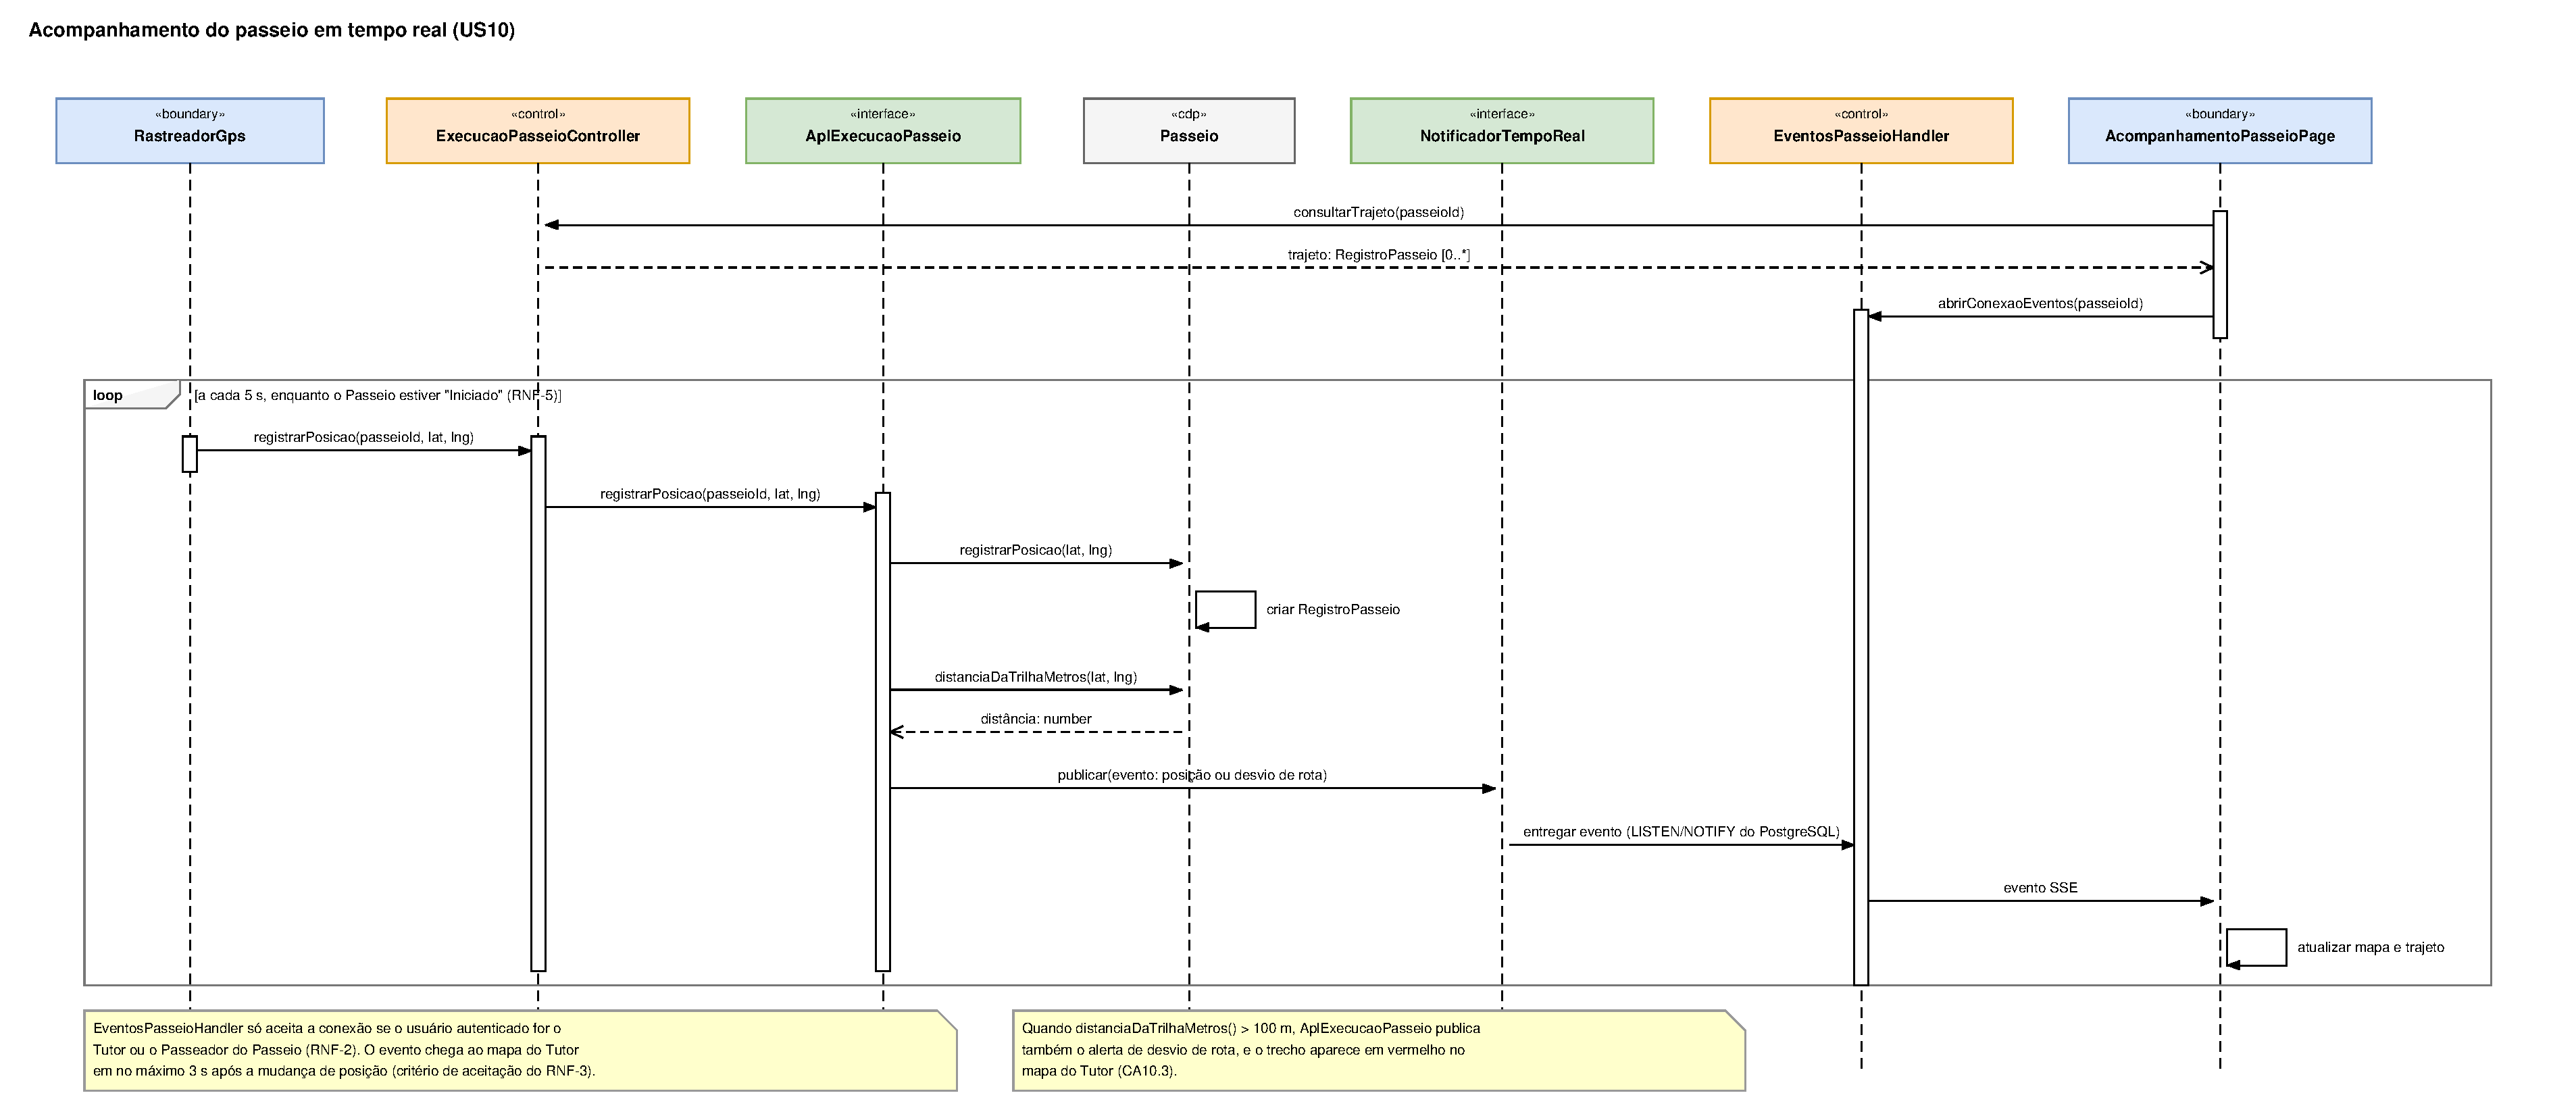
\includegraphics[angle=90,width=\textwidth,height=0.92\textheight,keepaspectratio]{figuras/ciu-servicos-seq-acompanhar.pdf}
	\caption{Diagrama de sequência do acompanhamento do passeio em tempo real.}
	\label{figura-ciu-seq-acompanhar}
\end{figure}


%=======================================================================================================
\FloatBarrier
\section{Subsistema Suporte}
\label{sec-ihc-suporte}

A Figura~\ref{figura-ciu-suporte} mostra o projeto da Camada de Interface com o Usuário do subsistema Suporte, juntamente com as classes de aplicação do \texttt{cgt} (Figura~\ref{figura-ln-suporte-cgt}). As telas correspondem às Figuras 25 a 30 do documento de requisitos. A Tabela~\ref{tabela-ciu-suporte} lista as páginas e os controladores.

\begin{figure}[h]
	\centering
	\figciu{figuras/ciu-suporte.png}{0.8}
	\caption{Projeto da Camada de Interface com o Usuário (\texttt{cih} e \texttt{cci}) do subsistema Suporte.}
	\label{figura-ciu-suporte}
\end{figure}

\begin{scriptsize}
\setlength{\tabcolsep}{3pt}
\begin{longtable}{|p{4.2cm}|p{3.6cm}|p{1.7cm}|p{1.3cm}|p{3.8cm}|}
	\caption{Páginas do subsistema Suporte.}
	\label{tabela-ciu-suporte}\\\hline
	\rowcolor{lightgray}
	\textbf{Página} & \textbf{Rota} & \textbf{Perfil} & \textbf{US} & \textbf{Controlador} \\\hline
	\endfirsthead
	\hline
	\rowcolor{lightgray}
	\textbf{Página} & \textbf{Rota} & \textbf{Perfil} & \textbf{US} & \textbf{Controlador} \\\hline
	\endhead
	\texttt{AbrirChamadoPage} & \texttt{/suporte/novo} & Tutor, Passeador & US16 & \texttt{Chamado\-Controller} \\\hline
	\texttt{MeusChamadosPage} & \texttt{/suporte} & Tutor, Passeador & US16 & \texttt{Chamado\-Controller} \\\hline
	\texttt{DetalheChamadoPage} & \texttt{/suporte/\allowbreak [protocolo]} & Tutor, Passeador & US16 & \texttt{Chamado\-Controller} e \texttt{EventosSuporte\-Handler} \\\hline
	\texttt{FilaAtendimentoPage} & \texttt{/atendimento/\allowbreak chamados} & Atendente & US17 & \texttt{Atendimento\-Controller} e \texttt{EventosSuporte\-Handler} \\\hline
	\texttt{AtendimentoChamadoPage} & \texttt{/atendimento/\allowbreak chamados/[id]} & Atendente & US17 & \texttt{Atendimento\-Controller} \\\hline
\end{longtable}
\end{scriptsize}

\begin{sloppypar}
\texttt{ChamadoController} se liga a \texttt{AplChamado}, e \texttt{AtendimentoController} a \texttt{AplAtendimento}. \texttt{EventosSuporteHandler} é um \textit{Route Handler} que, como \texttt{EventosPasseioHandler}, não chama operações do \texttt{cgt}: ele só assina os eventos que \texttt{AplChamado} e \texttt{AplAtendimento} publicam em \texttt{NotificadorTempoReal} e os repassa por SSE às páginas abertas. As funcionalidades do subsistema são:

\begin{itemize}
	\item \textbf{Abertura de chamado:} \texttt{AbrirChamadoPage} pede o tipo do problema (lista de seleção), a descrição, os anexos (fotos e capturas de tela) e, quando o problema aconteceu em um passeio, o passeio relacionado. Os dados vão a \texttt{ChamadoController}, que chama \texttt{abrirChamado()}. O tipo e a descrição são obrigatórios (CA16.1). Em caso de sucesso, o controlador redireciona para \texttt{DetalheChamadoPage}, que mostra o protocolo gerado e o status ``Em análise'' (CA16.2). Para chamados de ``Emergência'', a página destaca o tipo, e \texttt{AplChamado} publica o evento em \texttt{NotificadorTempoReal}, que o leva à fila do Atendente. \texttt{MeusChamadosPage} tem um \textit{link} para esta página;
	\item \textbf{Consulta dos chamados:} \texttt{MeusChamadosPage} lista os chamados do usuário (\texttt{listarMeusChamados()}), com protocolo, tipo e status. Ao escolher um deles, \texttt{DetalheChamadoPage} mostra o chamado e as respostas do Atendente (\texttt{consultarChamado()}). Quando o Atendente responde, \texttt{AplAtendimento} publica o evento em \texttt{NotificadorTempoReal}, e \texttt{DetalheChamadoPage}, conectada a \texttt{EventosSuporteHandler}, mostra a resposta sem recarregar a página (CA16.3);
	\item \textbf{Fila de atendimento:} \texttt{FilaAtendimentoPage} lista os chamados abertos (\texttt{listarFilaAtendimento()}), com os de ``Emergência'' em destaque e no topo, e mostra para cada um o tempo de espera. A página também mostra o indicador de primeiro atendimento em até 30 minutos (\texttt{calcularIndicadorAtendimento()}, RNF-4). A página recebe novos chamados por \texttt{EventosSuporteHandler}, sem o Atendente precisar recarregá-la;
	\item \textbf{Atendimento do chamado:} \texttt{AtendimentoChamadoPage} mostra (\texttt{consultarChamado()}) a descrição, o passeio relacionado, os anexos (que o Atendente pode visualizar ou baixar, CA17.3) e as respostas anteriores. O Atendente escreve a resposta (\texttt{responderChamado()}), o que muda o status para ``Em atendimento'', e pode encerrar o chamado com confirmação (\texttt{encerrarChamado()}), mudando o status para ``Resolvido''. Depois de responder, o Atendente continua na própria página; depois de encerrar, o controlador volta para \texttt{FilaAtendimentoPage}.
\end{itemize}
\end{sloppypar}


%=======================================================================================================
\FloatBarrier
\section{Padrões de Projeto na Camada de Apresentação}
\label{sec-ihc-padroes}

Além do MVC, foram usados padrões de projeto~\cite{falbo:notas18} na Camada de Apresentação:

\begin{itemize}
	\item \textbf{Observador (\textit{Observer}):} as páginas de acompanhamento do passeio, de fila de atendimento e de chamados são observadoras dos eventos publicados por \texttt{NotificadorTempoReal}. O navegador se inscreve por meio de um \texttt{EventSource}, conectado a \texttt{EventosPasseioHandler} ou a \texttt{EventosSuporteHandler}, e é avisado das mudanças, em vez de consultar o servidor de tempos em tempos (RNF-3);
	\item \textbf{Decorador (\textit{Decorator}):} os \textit{layouts} do Next.js envolvem as páginas de cada área (Tutor, Passeador e Atendente) com o menu, o cabeçalho e a verificação de sessão e de perfil, de modo que a estrutura visual e o controle de acesso não são repetidos em cada página;
	\item \textbf{Comando (\textit{Command}):} cada \textit{Server Action} representa um comando do usuário (por exemplo, agendar, cancelar, aceitar, responder), recebe os dados do formulário e devolve o resultado da operação, o que mantém um controlador pequeno e focado em uma tarefa.
\end{itemize}